%%%%%%%%%%%%%%%%%%%%%%% file template.tex %%%%%%%%%%%%%%%%%%%%%%%%%
%
% This is a general template file for the LaTeX package SVJour3
% for Springer journals.          Springer Heidelberg 2010/09/16
%
% Copy it to a new file with a new name and use it as the basis
% for your article. Delete % signs as needed.
%
% This template includes a few options for different layouts and
% content for various journals. Please consult a previous issue of
% your journal as needed.
%
%%%%%%%%%%%%%%%%%%%%%%%%%%%%%%%%%%%%%%%%%%%%%%%%%%%%%%%%%%%%%%%%%%%
%
% First comes an example EPS file -- just ignore it and
% proceed on the \documentclass line
% your LaTeX will extract the file if required
\begin{filecontents*}{example.eps}
%!PS-Adobe-3.0 EPSF-3.0
%%BoundingBox: 19 19 221 221
%%CreationDate: Mon Sep 29 1997
%%Creator: programmed by hand (JK)
%%EndComments
gsave
newpath
  20 20 moveto
  20 220 lineto
  220 220 lineto
  220 20 lineto
closepath
2 setlinewidth
gsave
  .4 setgray fill
grestore
stroke
grestore
\end{filecontents*}
%
\RequirePackage{fix-cm}
%
\documentclass{svjour3}                     % onecolumn (standard format)
%\documentclass[smallcondensed]{svjour3}     % onecolumn (ditto)
%\documentclass[smallextended]{svjour3}       % onecolumn (second format)
%\documentclass[twocolumn]{svjour3}          % twocolumn
%
\smartqed  % flush right qed marks, e.g. at end of proof

% Insert the name of "your journal" with
\journalname{Shock Waves}
%

\usepackage{setspace}
\usepackage{graphicx}
\graphicspath{{../Figures/}}
\usepackage{epsfig}
\usepackage{color}
\usepackage{psfrag}

%\usepackage{subfigure}
%\usepackage{subfig}
%\usepackage{tabularx}
\usepackage{subfigmat}
\usepackage{subeqnarray}
\usepackage[colorlinks]{hyperref}
\usepackage{amsmath,amsfonts,amsfonts}
\usepackage{xcolor,colortbl}
\usepackage[mathscr]{euscript}
\usepackage{algorithm2e}
\usepackage{siunitx}
\usepackage{rotating}
\usepackage{bm,bbm}
\setcounter{secnumdepth}{3}
\usepackage[version=3]{mhchem}   % chemistry package
\usepackage[numbers]{natbib}
\usepackage{optidef}
\usepackage[T1]{fontenc}
%additional commands
%
%%%%%%%%%%%%%%%%%%%%%%%%%%%%%%%%%%%%%%%%%%%%%%%%%%%%%%%%%%%%%%%%%%%%%%
%
\makeatletter
\newcommand\rlarrows{\mathop{\operator@font \rightleftarrows}\nolimits}
\makeatother
%
%%%%%%%%%%%%%%%%%%%%%%%%%%%%%%%%%%%%%%%%%%%%%%%%%%%%%%%%%%%%%%%%%%%%%%

%\newcommand{\comment}[1]{{\color{blue} \bf [#1]}}
\newcommand{\comment}[1]{{\color{blue} #1}}

\newenvironment{itemizePacked}{
\begin{itemize}
  \setlength{\itemsep}{1pt}
  \setlength{\parskip}{0pt}
  \setlength{\parsep}{0pt}
}{\end{itemize}}
\newenvironment{enumeratePacked}{
\begin{enumerate}
  \setlength{\itemsep}{5pt}
  \setlength{\parskip}{0pt}
  \setlength{\parsep}{0pt}
}{\end{enumerate}}
% abbreviations %%%%%%%%%%%%%%%%%%%%%%%%%%%%%%%%%%%%%%%%%%%%%%%%%%%%%%
%
%\def\codefont{scriptsize}
\newcommand{\f}[2]{{\frac{#1}{#2}}}
\newcommand{\wt}[1]{{\widetilde{#1}}}
\newcommand{\wh}[1]{{\widehat{#1}}}
\newcommand{\wc}[1]{{\widecheck{#1}}}
\newcommand{\chem}[1]{\ensuremath{\mathrm{#1}}}
\newcommand{\lrangle}[1]{{\langle{#1}\rangle}}
\newcommand{\lrcurl}[1]{{\{{#1}\}}}
\newcommand{\ol}[1]{{\overline{#1}}}
%\newcommand{\ul}[1]{{\underline{#1}}}
\newcommand{\tr}{{\scriptscriptstyle\mathsf T}}
\newcommand{\dd}{{\scriptscriptstyle\Delta}}
\newcommand{\eps}{{\varepsilon}}

\def\RPP{reaction progress parameter}

% boldface-italic font
\newcommand{\bfit}[1]{\textbf{\textit{#1}}}

%
% SOME COLORS %%%%%%%%%%%%%%%%%%%%%%%%%%%%%%%%%%%%%%%%%%%%%%%%%%%%%%%%
%
\newcommand{\colred}[1]{{\color{red} #1}}
\newcommand{\colblue}[1]{{\color{blue} #1}}
\newcommand{\colwhite}[1]{{\color{white} #1}}
\newcommand{\colgreen}[1]{{\color{green} #1}}
\newcommand{\colbrown}[1]{{\color{Brown} #1}}
\newcommand{\colfucsia}[1]{{\color{Fuchsia} #1}}
\newcommand{\colBlue}[1]{{\color{Blue} #1}}
\newcommand{\corrections}[1]{{\color{blue}#1}}
%
% FOR COMBUSTION TEXT %%%%%%%%%%%%%%%%%%%%%%%%%%%%%%%%%%%%%%%%%%%%%%%%
%
\def\chist{\chi_{Z,\up{st}}}
\def\chiq{\chi_{Z,\up{q}}}
\def\chii{\chi_{Z,\up{i}}}
%
% Standard TEX-abbreviations used %%%%%%%%%%%%%%%%%%%%%%%%%%%%%%%%%%%%
%
\def\cldbpage{\clearpage{\pagestyle{empty}\cleardoublepage}}
%
% CALIGRAPHICAL SYMBOLS %%%%%%%%%%%%%%%%%%%%%%%%%%%%%%%%%%%%%%%%%%%%%%
%
\def\cA{{\cal{A}}}
\def\cB{{\cal{B}}}
\def\cC{{\cal{C}}}
\def\cO{{\cal{O}}}
\def\cD{{\cal{D}}}
\def\cE{{\cal{E}}}
\def\cF{{\cal{F}}}
\def\cH{{\cal{H}}}
\def\cJ{{\cal{J}}}
\def\cG{{\cal{G}}}
\def\cN{{\cal{N}}}
\def\cL{{\cal{L}}}
\def\cS{{\cal{S}}}
\def\cT{{\cal{T}}}
\def\cU{{\cal{U}}}
\def\cC{{\cal{C}}} 
\def\cZ{{\cal{Z}}}
\def\cM{{\cal{M}}}
\def\cP{{\cal{P}}}
\def\cR{{\cal{R}}}
\def\cV{{\cal{V}}}
\def\cQ{{\cal{Q}}}
%
% NEW FUNCTION NAMES %%%%%%%%%%%%%%%%%%%%%%%%%%%%%%%%%%%%%%%%%%%%%%%%%
%
\def\erf{{\rm{erf}}}
%
% TEXT FONT DEFINITIONS %%%%%%%%%%%%%%%%%%%%%%%%%%%%%%%%%%%%%%%%%%%%%%
%
\def\up{\textup}
\def\p{\partial}
\def\d{\textup d}
\def\D{\displaystyle}
%\def\S{\scriptsize}
\def\OmFint{\iiint\limits_{\OmF}}
\def\OmF{{\Omega_{\cal F}}}
\def\OmA{{\Omega_{\cal A}}}
\def\e{\textup{e}}
\def\i{\textup{i}}
\def\REFUP{\rm{ref}}
\def\REF{_{\REFUP}}
%
% DIMENSIONLESS QUANTITIES %%%%%%%%%%%%%%%%%%%%%%%%%%%%%%%%%%%%%%%%%%%
%
%\def\Re{{\rm{Re}}}
\def\Fr{{\rm{Fr}}}
\def\M{{\rm{M}}}
\def\Ce{{\rm{Ce}}}
\def\Re{{\rm{Re}}}
\def\Rd{{\rm{Rd}}}
\def\Le{{\rm{Le}}}
\def\Da{{\rm{Da}}}
\def\Ka{{\rm{Ka}}}
\def\Nu{{\rm{Nu}}}
\def\Sc{{\rm{Sc}}}
\def\Ri{{\rm{Ri}}}
\def\Ec{{\rm{Ec}}}
\def\Tu{{\rm{Tu}}}
\def\St{{\rm{St}}}
\def\Mi{{\rm{Mi}}}
\def\Ra{{\rm{Ra}}}
\def\Ze{{\rm{Ze}}}
%
% FOR LATEX %%%%%%%%%%%%%%%%%%%%%%%%%%%%%%%%%%%%%%%%%%%%%%%%%%%%%%%%%%
%
 \def\avec{{\mbox{\boldmath$a$}}}
 \def\bvec{{\mbox{\boldmath$b$}}}
 \def\Bvec{{\mbox{\boldmath$B$}}}
 \def\cvec{{\mbox{\boldmath$c$}}}
 \def\dvec{{\mbox{\boldmath$d$}}}
 \def\evec{{\mbox{\boldmath$e$}}}
 \def\Fvec{{\mbox{\boldmath$F$}}}
 \def\Nvec{{\mbox{\boldmath$N$}}}
 \def\fvec{{\mbox{\boldmath$f$}}}
 \def\gvec{{\mbox{\boldmath$g$}}}
 \def\hvec{{\mbox{\boldmath$h$}}}
 \def\ivec{{\mbox{\boldmath$i$}}}
 \def\jvec{{\mbox{\boldmath$j$}}}
 \def\kvec{{\mbox{\boldmath$k$}}}
 \def\pvec{{\mbox{\boldmath$p$}}}
 \def\Pvec{{\mbox{\boldmath$P$}}}
 \def\uvec{{\mbox{\boldmath$u$}}}
 \def\Uvec{{\mbox{\boldmath$U$}}}
 \def\nvec{{\mbox{\boldmath$n$}}}
 \def\tvec{{\mbox{\boldmath$t$}}}
 \def\Rvec{{\mbox{\boldmath$R$}}}
 \def\rvec{{\mbox{\boldmath$r$}}}
 \def\svec{{\mbox{\boldmath$s$}}}
 \def\Svec{{\mbox{\boldmath$S$}}}
 \def\xvec{{\mbox{\boldmath$x$}}}
 \def\vvec{{\mbox{\boldmath$v$}}}
 \def\wvec{{\mbox{\boldmath$w$}}}
 \def\yvec{{\mbox{\boldmath$y$}}}
 \def\mvec{{\mbox{\boldmath$m$}}}
 \def\Xvec{{\mbox{\boldmath$X$}}}
 \def\qvec{{\mbox{\boldmath$q$}}}
 \def\0vec{{\mbox{\boldmath$0$}}}
 \def\xivec{{\mbox{\boldmath$\xi$}}}
 \def\rhovec{{\mbox{\boldmath$\rho$}}}
 \def\wpvec{{\boldsymbol{\wp}}}
 \def\psivec{{\mbox{\boldmath$\psi$}}}
 \def\epsvec{{\mbox{\boldmath$\epsilon$}}}
 \def\phivec{{\mbox{\boldmath$\phi$}}}
 \def\varphivec{{\mbox{\boldmath$\varphi$}}}
 \def\zetavec{{\mbox{\boldmath$\zeta$}}}
 \def\kappavec{{\mbox{\boldmath$\kappa$}}}
 \def\varkappavec{{\pmb{\varkappa}}}
 \def\etavec{{\mbox{\boldmath$\eta$}}}
 \def\Psivec{{\boldsymbol{\Psi}}}
 \def\Phivec{{\boldsymbol{\Phi}}}
 \def\Wvec{{\boldsymbol{W}}}
 \def\Yvec{{\mbox{\boldmath$Y$}}}
 \def\Vvec{{\mbox{\boldmath$V$}}}
 \def\cLvec{{\boldsymbol{\cal{L}}}}
 \def\cMvec{{\boldsymbol{\cal{M}}}}
 \def\omegavec{{\mbox{\boldmath$\omega$}}}
 \def\Omegavec{{\mbox{\boldmath$\Omega$}}}
 \def\sigmavec{{\boldsymbol{\sigma}}}
 \def\Amat{{\underline{\underline{{A}}}}}
 \def\Bmat{{\underline{\underline{{B}}}}}
 \def\Phimat{{\underline{\underline{{\Phi}}}}}
 \def\taumat{{\underline{\underline{{\tau}}}}}
 \def\sigmamat{{\underline{\underline{{\sigma}}}}}
 \def\Cmat{{\underline{\underline{{C}}}}}
 \def\Imat{{\underline{\underline{{I}}}}}
 \def\Jmat{{\underline{\underline{{J}}}}}
 \def\Smat{{\underline{\underline{{S}}}}}
 \def\Rmat{{\underline{\underline{{R}}}}}
 \def\Tmat{{\underline{\underline{{T}}}}}
 \def\Emat{{\underline{\underline{{E}}}}}
 \def\tmat{{\underline{\underline{{t}}}}}

 \def\alphavec{{\boldsymbol{\alpha}}}
 \def\betavec{{\boldsymbol{\beta}}}
 \def\tauvec{{\boldsymbol{\tau}}}
 \def\thetavec{{\boldsymbol{\theta}}}
 \def\lambdavec{{\mbox{\boldmath$\lambda$}}}
 \def\cTmat{{\underline{\underline{{\cal{T}}}}}}
 \def\cLmat{{\underline{\underline{{\cal{L}}}}}}
 \def\cMmat{{\underline{\underline{{\cal{M}}}}}}
 \def\kappamat{{\underline{\underline{{\kappa}}}}}
%
% Grad, Div, ... %%%%%%%%%%%%%%%%%%%%%%%%%%%%%%%%%%%%%%%%%%%%%%%%%%%%%
%
\def\Grad{\nabla}
\def\Div{\nabla \cdot}
\def\Lap{\nabla^2}
%
%% Short cuts
\newcommand{\Ar}{\Theta}
\newcommand{\tign}{\tau_{\mathrm{ign}}}
\newcommand{\stnshk}{{\textsc{StanShock}}}
\newcommand{\cantera}{{\sc{Cantera}}}
\newcommand{\python}{{\sc{Python}}}
\def\indicator{{\mathbf{1}}}
\usepackage[greek,english]{babel}
\newcommand{\change}{\text{\greektext D}}
\newcommand{\flux}{\mathbf{f}}
\newcommand{\approxFlux}{\hat{\mathbf{f}}}
\newcommand{\reals}{\mathbbm{R}}
\newcommand{\integers}{\mathbbm{Z}}
\newcommand{\ones}{\mathbf{1}}
\newcommand{\mdotpp}{\dot{m}^{\prime\prime}}
\newcommand{\Up}{u^{*,\prime}_5} 
\newcommand{\U}{(U^*_\mathrm{s2}+u^*_5)}
\newcommand{\T}{T^*_5}
\newcommand{\Tp}{T^{*,\prime}_5}
\newcommand{\DOne}{\frac{\mathrm{d}}{\mathrm{d}y^*}}
\newcommand{\DTwo}{\frac{\mathrm{d}^2}{\mathrm{d}y^{*,2}}}
\renewcommand{\M}{\mathrm{M}}
\newcommand{\Expect}{\mathbbm{E}}
\newcommand{\Prob}{\mathbbm{P}}
\newcommand{\pd}[2]{\frac{\partial #1}{\partial #2}}
\newcommand{\pdTwo}[2]{\frac{\partial^2 #1}{\partial #2^2}}
\renewcommand{\u}{\mathbf{u}}
\newcommand{\Y}{\mathbf{Y}}
\newcommand{\w}{\dot{\omega}^{\prime\prime\prime}}


\begin{document}

\title{\textbf{\stnshk}: A Gasdynamic Model for Shock Tube Simulations with Non-ideal Effects and Chemical Kinetics}
\titlerunning{\stnshk}
\author{Kevin Grogan         \and
        Matthias Ihme
}


\institute{K. Grogan \at
	ATA Engineering, Inc. \\
	\email{kevin.grogan@ata-e.com} \and
	M. Ihme \at
	Stanford University \\
	\email{mihme@stanford.edu}
}

\date{Received: date / Accepted: date}
% The correct dates will be entered by the editor


\maketitle

\begin{abstract}
A high-order, quasi one-dimensional, reacting, compressible flow solver is developed to simulate non-ideal effects and chemical kinetics in shock tube systems. To this end, physical models for the thermoviscous boundary-layer development, area variation, gas interfaces, and reaction chemistry are considered. The model is first verified through simulations of steady isentropic nozzle flow, multispecies Sod's problem, laminar premixed flame, and ZND detonation test cases. Comparisons with experiments are performed by examining end-wall pressure traces that are gathered from shock tube experiments designed to test the code's capabilities. Subsequently, the solver is utilized for uncertainty quantification and design optimization of a driver insert. Both applications prove to be highly efficient indicating the utility of the solver for the design of experiments in consideration of non-ideal gas-dynamic effects.
\keywords{Shock tube \and Combustion \and Non-ideal Effects \and Optimization \and Uncertainty Quantification}
\end{abstract}
%%%%%%%%%%%%%%%%%%%%%%%%%%%%%%%%%%%%%%%%%%%%%%%%%%%%%%%%%%%%%%%%%%%%%%%%%%%%%%%%%%%%%%%%%%%%%%%%%%%%%%%%%%%%%%%%%%%%
\section{Introduction}
\label{SEC_INTRO}
	Shock tube  facilities remain invaluable for providing detailed information 
	about ignition delay times, extinction limits, and species time histories for the development of chemical kinetic mechanisms~\cite{HANSON_PECS2014}. These measurements are employed in the validation of chemical models and the characterization of new fuel mixtures. A shock tube is a long pipe, which is divided into a driver section and a driven section by a diaphragm. The driver section is pressurized with an inert gas, and the driven section contains the test gas mixture that is under experimental investigation. Following the rupture of the diaphragm,
	a normal shock develops which propagates into the driven section and is reflected at the end wall.
	
	Shock tubes rely on gas dynamic simplicity to study chemical kinetics with high accuracy. Under ideal conditions, the test gas mixture 
	in the region behind the reflected shock is stationary and uniform. However, non-ideal gas dynamics can significantly affect the ignition characteristics~\cite{PETERSEN_HANSON_SW2001}. A particularly pervasive non-ideality in shock tube experiments is an unsteady rise in test pressure, which in turn affects the measured reaction. For instance, Pang~\emph{et al.}~\cite{PANG_DAVIDSON_HANSON_PCI32} found a pressure rise at the a rate of 2\% per millisecond, which could be consequential for long ignition delay time measurements.
	
	
	The pressure rise is due to boundary layer displacement. Specifically, as the boundary layer develops, the core gas of the shock tube is compressed by the decreasing effective volume of the shock tube yielding the increase in pressure. For practical applications, this effect can be mitigated by employing large shock tube diameters, reducing the test time, and using driver inserts~\cite{DAVIDSON_HANSON_SW2009}. In particular, driver inserts cause the expansion wave behind the incident shock to be reflected towards the shock counteracting the observed pressure rise in turn. While driver inserts have successfully been employed to reduce the pressure rise in the test section, thereby extending the operable range of the shock tube~\cite{HONG_PANG_VASU_DAVIDSON_HANSON_SW2009}, their design for an experiment is an iterative and time-consuming process.  
	
Simple models such as {\sc{Chemshock}}~\cite{LI_OWENS_DAVIDSON_HANSON_IJCK2008} and the VTIM (volume as a function of time) reactor model~\cite{CHAOS_DRYER_IJCK2010} were developed to consider effects of the pressure rise of realistic shock tube systems in homogeneous reactor models. They both work by directly incorporating pressure measurements from shock tube experiments and isentropically correcting the temperature ({\sc{Chemshock}}) or volume (VTIM). By incorporating pressure measurements into zero-dimensional simulations, these models were found to improve the agreement with experimental data; however, they incorporate boundary layer effects and other non-idealities in an~\emph{a posteriori} manner. As such, their use is limited in the design of experiments since they do not represent the underlying physical processes.
	
	While gas-dynamic effects due to shock-boundary-layer-interaction may be captured through detailed, multidimensional simulations~\cite{WEBER_ORAN_BORIS_ANDERSON_POF1995,YAMASHITA_CF12,GROGAN_PCI2015,Khokhlov_ICDERS15,GROGAN_PCI2017,LIPKOWICZ_SW2018}, the computational currently prohibits the simulation of entire shock tube systems, the incorporation of detailed chemical mechanisms, or the examination of complex geometries. Hence, a computationally efficient and accurate model is necessary to study shock tube ignition for these purposes. 
	
	The purpose of this work is to propose, verify, validate, and apply a low-order model for shock tube ignition in the presence of non-ideal gas dynamics. To this end, a quasi one-dimensional model (\stnshk) is developed. The underlying mathematical model is presented in Sec.~\ref{SEC_MODEL}, a description of the verification and validation tests performed is contained in Sec.~\ref{SEC_VV}, and applications of the model to design optimization and uncertainty quantification are given in Sec.~\ref{SEC_APPLICATIONS}.
%%%%%%%%%%%%%%%%%%%%%%%%%%%%%%%%%%%%%%%%%%%%%%%%%%%%%%%%%%%%%%%%%%%%%%%%%%%%%%%%%%%%%%%%%%%%%%%%%%%%%%%%%%%%%%%%%%%%%%%%%%%%%%%%%%%%%%%%%%%%%%%%%%%%%%%%%%%%%%%%%%%%%%%%%%%%%%%%%%
\section{Model}\label{SEC_MODEL}

To motivate the \stnshk\ model, Fig.~\ref{FIG_STPHYS} illustrates the relevant physical processes in a shock tube. The modeling of these processes requires the consideration of complex shock wave dynamics, involving the development, propagation, reflection and self-interaction. Furthermore, since the driver gas is often much lighter than the driven gas to minimize the interaction of the reflected shock with the contact surface~\cite{HANDBOOK_OF_SHOCKWAVES}, a model for the material interface is required. Many shock tubes utilize a larger driver section area than driven section area to produce stronger incident shocks~\cite{ALPHER_JFM58}. Driver inserts~\cite{HONG_PANG_VASU_DAVIDSON_HANSON_SW2009} can be employed to tailor the test pressure. Therefore, it is necessary for the model to incorporate area variation. Additionally, friction and heat transfer due to the boundary layer cause an unsteady test pressure, which requires additional modeling. Finally, a chemical kinetic model must be integrated into \stnshk\ to study the interaction of the gas dynamics with the reaction chemistry. 

\begin{figure}[!ht!]
	\begin{center}
		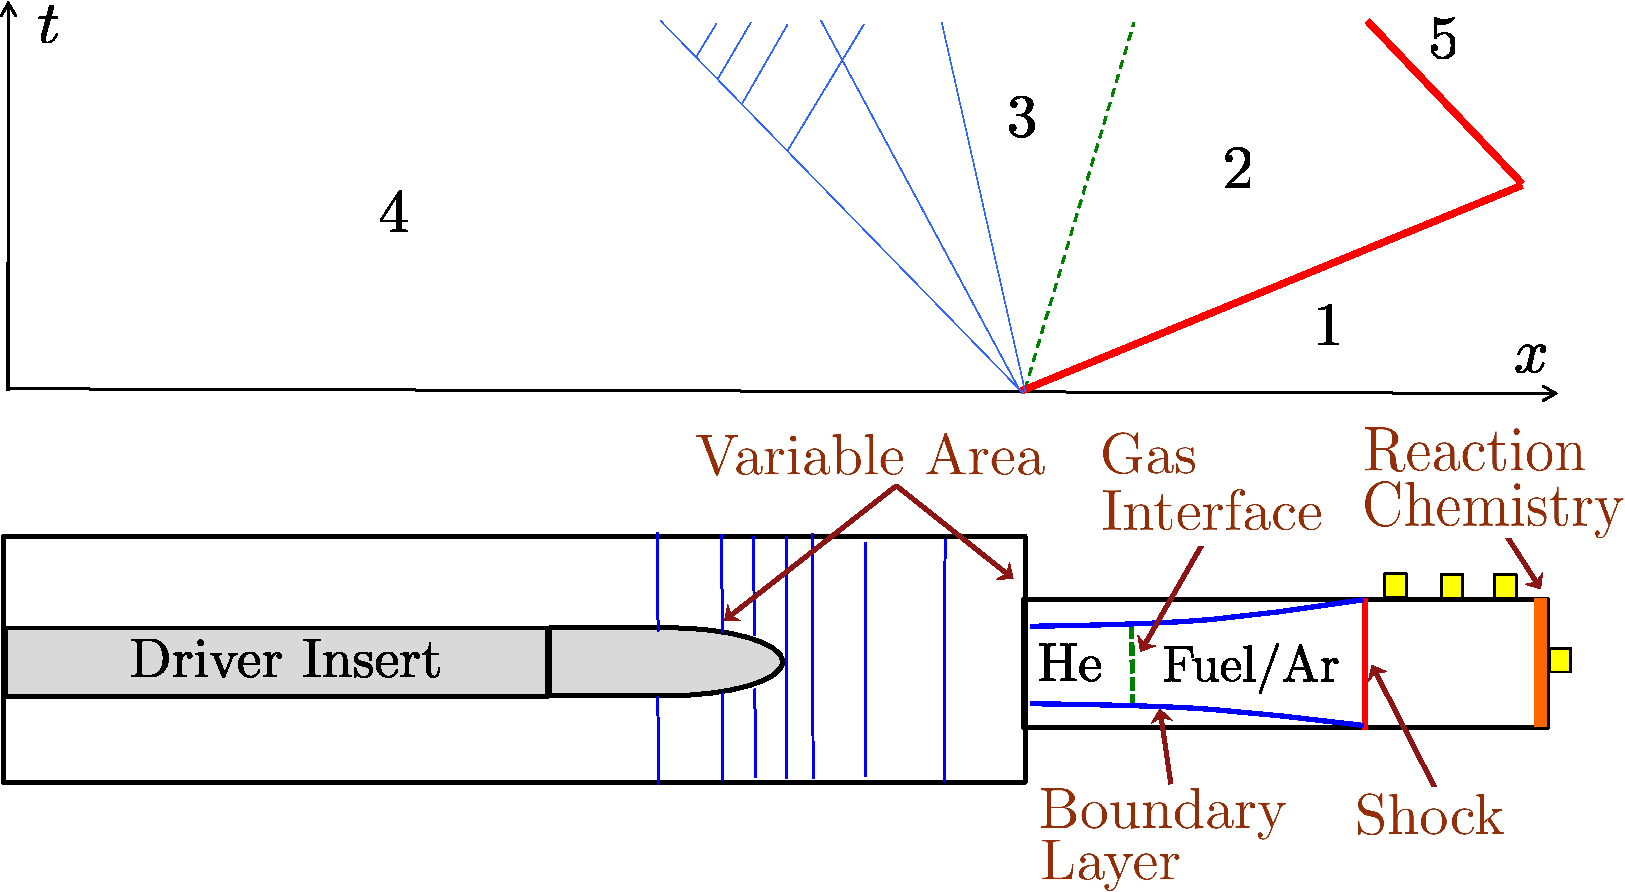
\includegraphics[width=84mm]{shockTubePhysics}
	\end{center}
	\caption{\label{FIG_STPHYS}Schematic illustration of relevant shock tube physics. An $x-t$ diagram is shown for reference with regions numbered in accordance to standard convention~\cite{HANDBOOK_OF_SHOCKWAVES}.}
\end{figure}

Following these requirements, the model equations employed in \stnshk\ are a quasi-one-dimensional formulation~\cite{SAAD_BOOK} of the Navier-Stokes equations with additional source terms for the reaction chemistry, area variation, and boundary layer development:
\begin{equation}\label{EQ_SS}
\f{\p \mathbf{q}}{\p t}+\f{\p }{\p x}(\mathbf{f}_\mathrm{i}-\mathbf{ f}_\mathrm{v}  )=\mathbf{s}_\mathrm{chem}+\mathbf{s}_\mathrm{area}+\mathbf{s}_\mathrm{bl}\ ,
\end{equation}
where 
\begin{equation}
	\mathbf{q}=\begin{bmatrix}
		\rho Y_1 \\
		\vdots\\
		\rho Y_{N}\\
		\rho u\\
		\rho e
	\end{bmatrix}\,,\quad 
	\mathbf{f}_\mathrm{i}=\begin{bmatrix}
	\rho Y_1u \\
	\vdots\\
	\rho Y_Nu\\
	\rho u^2+p\\
	\rho ue+pu
	\end{bmatrix}
	\,,\quad 
	\mathbf{f}_\mathrm{v}=\begin{bmatrix}
	\rho D_1\p_x Y_1 \\\
	\vdots\\
	\rho D_N\p_x Y_N\\
	\frac{4}{3}\mu \p_x u\\
	\lambda \p_x T
	\end{bmatrix}\ ,
\end{equation}
are the state-vector of conserved variables, inviscid flux, and viscous flux vectors, respectively. The energy, $e=e_\mathrm{s}+u^2/2$, contains the sensible and kinetic contributions, where $e_s=\int_{T_\mathrm{ref}}^T c_v\d T^\prime$ and $T_\mathrm{ref}$ is the reference temperature. Additionally, $D_n$, $\mu$, and $\lambda$ are the mass diffusion of the $n^\mathrm{th}$ species, dynamic viscosity, and thermal conductivity. The ideal gas equation of state is used to relate the pressure, density, temperature and composition: $p=\rho R T$, where $R=\mathcal{R}\sum_{n=1}^N Y_n/W_n$, $\mathcal{R}$ is the universal gas constant, and $W_n$ is the molecular weight of the $n^\mathrm{th}$ species. Note that for a single species, $Y_1=Y_N=1$, the $\mathbf{q}$, $\mathbf{f}_\mathrm{i}$, and $\mathbf{f}_\mathrm{v}$ terms of Eq.~\ref{EQ_SS} reduce to the one dimensional Navier-Stokes equations. 

The chemical source term is given by
\begin{equation}
	\mathbf{s}_\mathrm{chem} = \begin{bmatrix}
	\w_1 \\\
	\vdots\\
	\w_N\\
	0\\
	-\sum_{n=1}^N\Delta e_{\mathrm{f},n}^\circ(T_\mathrm{ref})\w_n
	\end{bmatrix}\ ,
\end{equation}
where $\Delta e_{\mathrm{f},n}^\circ(T_\mathrm{ref})$ is the formation energy at the reference temperature  of the $n^\mathrm{th}$ species, and $\w_n$ is the volumetric mass production rate of the $n^\mathrm{th}$ species. Furthermore, the area source terms are given by 
\begin{equation}
\label{EQ_SAREA}
\mathbf{s}_\mathrm{area}=
-\mathbf{q}\frac{\p\ln A}{\p t} -(\mathbf{f}_\mathrm{a}-p\hat{\mathbf{e}}_{N+1})\frac{\p\ln A}{\p x}\ ,
\end{equation}
where $A$ is the cross-sectional area, and $\hat{\mathbf{e}}_{N+1}$ is the unit vector corresponding to the momentum equation. The functional form of $A$ is known \emph{a priori}, and describes the geometry of the shock tube. Due to the presence of driver inserts, the cross-section of the shock tube is assumed to be annular with the hydraulic diameter, $D$, given by
\begin{equation}
D=D_\mathrm{o}-D_\mathrm{i} ,
\end{equation}
where $D_\mathrm{o}$ and $D_\mathrm{i}$ are the outer and inner diameters, respectively. Note that for sections of the shock tube without a driver insert, $D=D_\mathrm{o}$. Commonly, the term $\partial_t \ln A$ in Eq.~\ref{EQ_SAREA} will be zero; however, this term is implemented to enable the consideration of a finite opening time of the shock tube diaphragm.

Finally, the boundary layer source terms are modeled as 
\begin{equation}\label{EQ_BLSRC}
	\mathbf{s}_\mathrm{bl}=-\frac{4}{D}\begin{bmatrix}
		0\\
		\vdots\\
		0\\
		\tau\\
		q
	\end{bmatrix}
\end{equation}
where the shear stress at the wall is given by $\tau$, and the energy losses are given by $q$. The shear stress at the wall is related to the skin friction coefficient, $C_\mathrm{f}$, by
\begin{equation}
\label{EQ_TAU}
C_{\mathrm{f}}=\frac{\tau}{\frac{1}{2}\rho u^{2}}\; .
\end{equation}
In the current work, the skin-friction coefficient is obtained from the analytical solution for Poiseuille flow at low Reynolds numbers and the K\'arm\'an-Nikuradse relation at high Reynolds numbers~\cite{KAYS_BOOK2005}:

\begin{equation}
\label{EQ_CF}
C_\mathrm{f}=
\begin{cases}
{16}/{\Re}\ &\text{for}\ \Re<2300 \\
K(\Re)\ &\text{for}\ \Re\ge 2300
\end{cases}\ ,
\end{equation}
where the function $K(\cdot)$ is the solution of the implicit equation
\begin{equation}\label{EQ_KN}
\frac{1}{\sqrt{C_{\mathrm{f}}/2}}=2.46\ln\left(\mathrm{Re}\sqrt{C_{\mathrm{f}}/2}\right)+0.3\;\ ,
\end{equation}	
with respect to the skin friction coefficient. The use of Eq.~\ref{EQ_KN} presumes smooth walls for the shock tube and that the gap between a driver insert and the outer wall of the shock tube is well-described by this relation. The Reynolds number is based on the shock tube geometry and the local velocity:
\begin{equation}
\label{EQ_RED}
\Re=\f{\rho |u|L}{\mu}\; ,
\end{equation}
where the characteristic length scale, $L$, is defined as the hydraulic diameter
\begin{equation}
	L=\left(\frac{1+\indicator[D_i=0]}{2}\right)D
\end{equation}
where $\indicator[\cdot]$ is the indicator function. The switching via the indicator function is employed to assure that the asymptotic cases of no driver insert and large driver insert are treated with the appropriate length scale. Note that the absolute value of axial velocity is taken to yield a positive Reynolds number. Also, the sign of $\tau$ is adjusted to ensure that it remains in opposition to the flow and is set to zero when $u=0$. 

In a similar manner, the heat loss from the boundary layer is found with a Nusselt number correlation for internal flows with isothermal walls~\cite{KAYS_BOOK2005}:
\begin{equation}
\label{EQ_NU}
\Nu=
\begin{cases}
3.657 & \Re<2300 \\
0.021\Pr^{0.5}\Re^{0.8} & 2300\le\Re< 2\times 10^5\\
\frac{\Re\Pr(C_{\mathrm{f}}/2)}{0.88+13.39(\mathrm{Pr}^{2/3}-0.78)\sqrt{C_{\mathrm{f}}/2}} & 2\times 10^5\le \Re
\end{cases}\ ,
\end{equation}
where the Nusselt number relates to the heat loss by
\begin{equation}
q=\Nu\frac{\lambda}{L}(T-T_{\mathrm{w}}) ,
\end{equation}
and $T_{\mathrm{w}}$ is the wall temperature of the shock tube. The wall is assumed to be isothermal since the timescales of the chemical reactions and heating by shock compression are insufficient to cause an appreciable change in wall temperature~\cite{MARK_JAS1957}. However, at high Reynolds number, a relation for the constant heat flux is employed since the heat transfer becomes less sensitive to the boundary condition at high turbulence levels~\cite{KAYS_BOOK2005}.
%==============================================================================================================
\subsection{Numerical Method}
The numerical method used to solve Eq.~\ref{EQ_SS} is described subsequently. The choices of the numerical method are influenced by those made by other authors in the construction of  compressible reacting flow solvers~\cite{HOUIM_KUO_JCP_2011,ZIEGLER_THESIS11,LV_JCP2014}. Furthermore, the discretization schemes are selected to ensure numerical stability, to minimize computational expense, and to efficaciously incorporate the relevant shock tube gas dynamics and detailed reaction chemistry. This section proceeds with a discussion of the temporal integration, the model for the material surfaces, the flux calculation procedure, and the edge interpolation scheme.
%##########################################################################################################

\subsubsection{Spatial Discretization}
A fifth-order WENO scheme~\cite{SHU_REPORT1997, GROGAN_THESIS18} is chosen as the interpolator for the advective fluxes. The high-order scheme is motivated by the requirement to resolve the gas-dynamics with as few grid-points as possible. Furthermore, the TVD property of the scheme ensures that spurious oscillations do not severely affect the reaction chemistry near a shock. For the diffusive fluxes, a second-order central difference is utilized.

\subsubsection{Temporal Integration}
A splitting scheme is utilized to temporally integrate Eq.~\ref{EQ_SS}. In this method, the numerically stiff reaction chemistry is treated implicitly to reduce computational expense and coupled to the other terms via Strang splitting~\cite{GLOWINSKI_BOOK}. Furthermore, the non-stiff contributions by advection, diffusion, area variation, and boundary layer source terms utilize explicit time integration to avoid computing Jacobians. 

The advection terms are advanced using a third-order Runge-Kutta scheme~\cite{GROGAN_THESIS18}, which has been determined to be stable for Courant-Friedrichs-Lewy condition less than unity for the WENO scheme utilized~\cite{SHU_REPORT1997}. The boundary layer terms, area variation terms, and diffusive fluxes are forward integrated using Lie splitting to enhance the modularity of the solver. Furthermore, the implicit integration of the chemical source term is performed using the LSODE solver built-in to {\sc{scipy}}~\cite{SciPy}, while the reaction rates are evaluated via \cantera~\cite{Cantera}. 
%##########################################################################################################
\subsubsection{Flux Model}

Shock tube experiments often utilize differing driver and driven gases to tailor the incident shock wave. To account for this material interface, the double-flux model is employed~\cite{ABGRALL_JCP1996,ABGRALL_KARNI_JCP2001,BILLET_ABGRALL_JCP2003}. The double-flux model allows for the efficient computation of the approximate flux across contact discontinuities without spurious oscillations in pressure. The model requires the development of linear interpolation tables for the specific heats towards the computation of the energy, and the computation of two fluxes at each face in a ghost fluid method~\cite{GROGAN_THESIS18}. The linear interpolation tables are generated from a supplied \cantera\ solution object.

Consistency with the double-flux model requires adequate modeling of the contact surface. Hence, the low-dissipation Harten-Lax-van Leer-Contact (HLLC) flux for multi-species flows is utilized~\cite{TORO_BOOK,GROGAN_THESIS18}. The HLLC flux is an approximate solution to the Riemann problem for the Euler equations and is a three-wave flux model.
%##########################################################################################################
\subsubsection{Edge Interpolation}
The computation of the fluxes on the right and left edges of the cell requires the interpolation of the cell-averaged values for the characteristic variables to each edge. The flux computation utilizes the cell's specific heat ratio in accordance with the double-flux model. Additionally, it is noted that the double-flux model requires two flux computations per cell rather than one; however, this additional cost has been found to be negligible -- particularly for reacting simulations with detailed chemical kinetics, where the computational cost is dominated by the temporal integration of the reaction chemistry. 

After the characteristic variables are interpolated to the edges, they are transformed into conserved variables for use in the HLLC flux computation. While the use of the characteristic variables as interpolant increases the computational cost of the simulation, significant reductions in oscillations are found near discontinuities when compared to the use of primitive or conservative variables as the interpolant~\cite{HOUIM_KUO_JCP_2011}. 



%##########################################################################################################
\subsubsection{Implementation}
In order to yield a highly portable and modular code, \stnshk\ is written in object-oriented \python. The use of \python\ as programming language eases additional development for subsequent studies. Computationally intense portions of the code such as the thermodynamic property computations, WENO interpolation, and the HLLC flux evaluation are just-in-time compiled, which yields significant speed-up. 

A flow chart of typical operation of the code is shown in~\ref{FIG_FLOWCHART}. As indicated in the figure, a \python\ script is first used to set-up and run a \stnshk\ solution object. This object makes use of {\sc{Cantera}} as the thermochemistry software. At run time, the solution object is compiled using {\sc{Numba}}~\cite{Lam2015NumbaAL}. Subsequently, the \stnshk\ solution proceeds until the final time, $t_\mathrm{final}$, integrating the physical models selected by the user in the input script. Finally, the script may be post-processed using a graphical library such as matplotlib~\cite{Hunter_matplotlib_2007} as depicted in the figure. Built-in to the \stnshk\ solver is the capability to plot $x-t$ diagrams of the solution for selected flow variables.

\begin{figure}[!h!]
	\begin{center}
		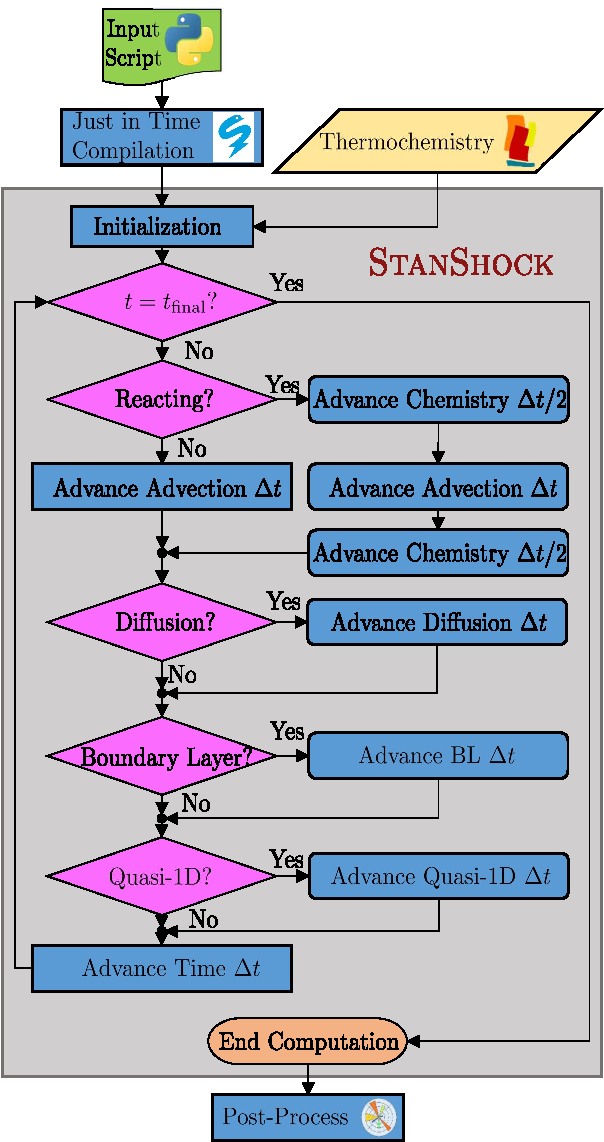
\includegraphics[width=70mm]{flowDiagram}
	\end{center}
	\caption{\label{FIG_FLOWCHART}Flow chart of typical operation of the \stnshk\ solver.}
\end{figure}
%%%%%%%%%%%%%%%%%%%%%%%%%%%%%%%%%%%%%%%%%%%%%%%%%%%%%%%%%%%%%%%%%%%%%%%%%%%%%%%%%%%%%%%%%%%%%%%%%%%%%%%%%%%%%%%%%%%%
\section{Verification and Validation}\label{SEC_VV}
The \stnshk\  solver requires verification of the numerical methods to ensure its intended operation. Furthermore, the predictive capabilities of \stnshk\ must be validated to ensure the utility of the solver. Hence, the subsequent section proceeds with verification cases including the advection of an analytical shock tube problem, isentropic nozzle flow, a laminar flame, and a Zeldovich-von Neumann-Doring detonation. Finally, a comparison of the solver with experimental data will be discussed.
\subsection{Analytical Shock Tube Problem}
Of great importance to \stnshk\ is its capability to reproduce an analytical shock tube flow absent of non-ideal effects. This assures the capability of \stnshk\ to model shock propagation, contact surfaces, and expansion waves; all of which are fundamental to the operation of shock tubes in chemical kinetic experiments. For this, the analytical solution to a multi-species Sod shock tube problem~\cite{SOD_JCP78,LV_JCP2014} is used as a test case.

The initial condition for the multi-species Sod's problem is a Riemann problem with a discontinuity in density, pressure, and specific heat ratio: 
\begin{subeqnarray}
	\rho(x,0)/\rho_4&=&\begin{cases}
		1\ \text{for}\ x/L<1/2 \\
		1/8\ \text{for}\ x/L\ge1/2
	\end{cases}\ , \\
	u(x,0)/c_4&=&0\ , \\
	p(x,0)/p_4&=&\begin{cases}
		1\ \text{for}\ x/L<1/2 \\
		1/10\ \text{for}\ x/L\ge1/2
	\end{cases}\ , \\
	\gamma(x,0)&=&\begin{cases}
		7/5\ \text{for}\ x/L<1/2 \\
		5/3\ \text{for}\ x/L\ge1/2
	\end{cases}\ ,
\end{subeqnarray}
where the subscript ``4'' follows shock tube conventions as shown in Fig.~\ref{FIG_STPHYS}, indicating the gas in the initial driver section state, and $c$ is the speed of sound. Details about the analytical solution to a Riemann problem for gas dynamics may be found in the monographs by Saad~\cite{SAAD_BOOK} or Laney~\cite{LANEY_BOOK}.  A comparison of the analytical solution to the numerical solution of \stnshk\ is shown in Fig.~\ref{FIG_SP}. The implemented scheme shows good agreement with the analytical solution. In particular, interfaces exhibit minimal oscillation, and the pressure remains constant across the contact surface in accordance with the double-flux model. The contact surface is shown to be somewhat diffuse. However, the sharpness of the contact discontinuity improves with increasing spatial resolution as shown in Fig.~\ref{FIG_SP_1000}. Hence, the results for the multi-species Sod shock tube problem verify that \stnshk\ is adequate for modeling gas dynamics with discontinuities.	
\begin{figure}[!h!]
	\centering
	\subfigure[\label{FIG_SP_100} $n_x=100$]{
		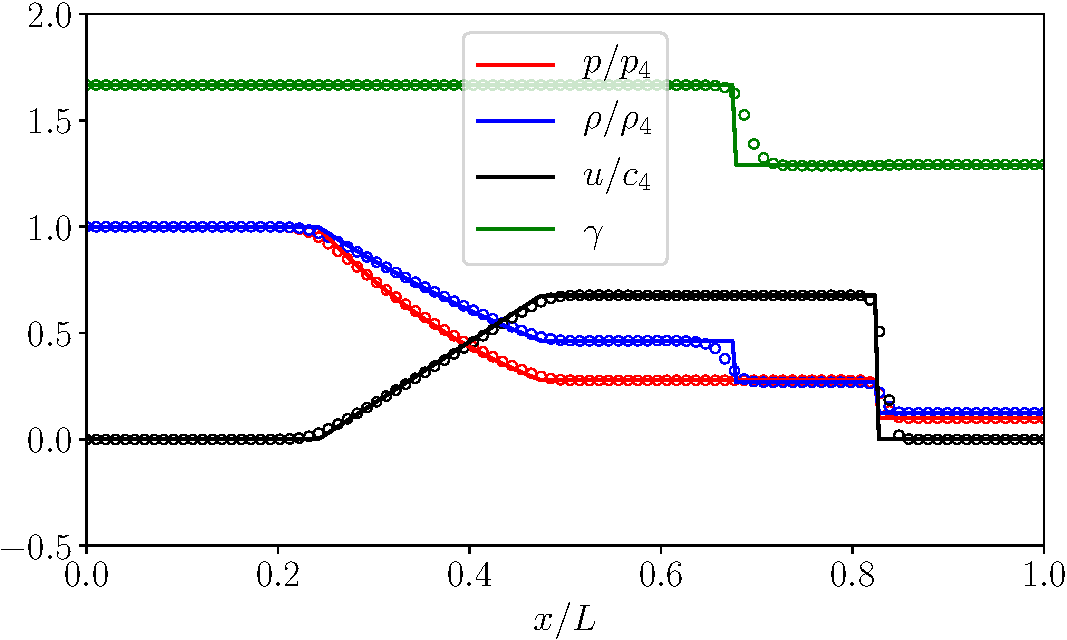
\includegraphics[width=84mm]{SodsProblem100}}
	\subfigure[\label{FIG_SP_1000} $n_x=1000$]{
		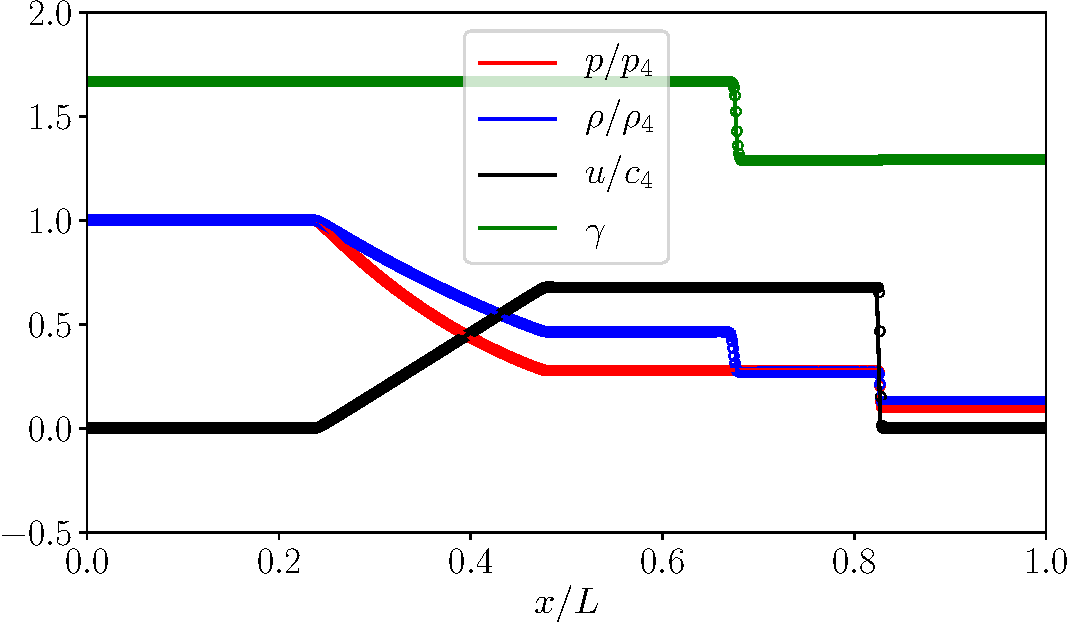
\includegraphics[width=84mm]{SodsProblem1000}}
	\caption{\label{FIG_SP} Comparison of the numerical ($\circ$) and analytical ($-$) solutions to a multicomponent version of Sod's problem~\cite{SOD_JCP78,LV_JCP2014} on a coarse and a fine grid. Snapshots are shown at $t=0.2L\sqrt{\rho_4/p_4}$.}
\end{figure}

\subsection{Isentropic Nozzle Flow}
Shock tubes are often designed with an enlarged driver cross section compared to that of the driver in order to strengthen the incident shock~\cite{ALPHER_JFM58}. Representing these geometric variations necessitates \stnshk's capability to model quasi-1D dimensional area changes. 

Verification of \stnshk's variable-area modeling capability is shown in Fig.~\ref{FIG_IN}. The test case is a smoothly-diverging, supersonic, isentropic nozzle with an area profile given by a sinusoid: 
\begin{equation}
	A(x)=\frac{1}{2}\left[3-\cos\left(\pi\frac{ x}{L}\right)\right]\;.
\end{equation} 
The analytical solution of this case is found via classical steady, one-dimensional, isentropic flow relations~\cite{SAAD_BOOK}:
\begin{subeqnarray}
	AM\left[\frac{2}{\gamma+1}\left(1+\frac{\gamma-1}{2}M^2\right)\right]^{-\frac{\gamma+1}{2(\gamma-1)}}&=&\mathrm{const.}\ ,\\
	\frac{p}{p_0}&=&\left(1+\frac{\gamma-1}{2}M^2\right)^{\frac{\gamma}{\gamma-1}}\ ,\\
	\frac{\rho}{\rho_0}&=&\left(\frac{p}{p_0}\right)^{\frac{1}{\gamma}}\ ,
\end{subeqnarray}
where $M$ is the Mach number, and the subscript "0" indicates the stagnation value. The inlet and outlet boundary conditions are supersonic, and the inflow state is $[T,M,p,\gamma]=[300\,\text{K},6/5 ,10^5\,\text{Pa},7/5]$. The domain is initialized to the inflow state and allowed to evolve temporally to a steady solution. Comparisons of simulation results and theoretical solutions are shown in Fig.~\ref{FIG_IN}. \stnshk\ is demonstrated to accurately reproduce the analytical solution for the flow quantities. Hence, \stnshk\ is verified to reproduce the analytical solution of quasi-1D gas dynamics.
\begin{figure}[!ht!]
	\centering
	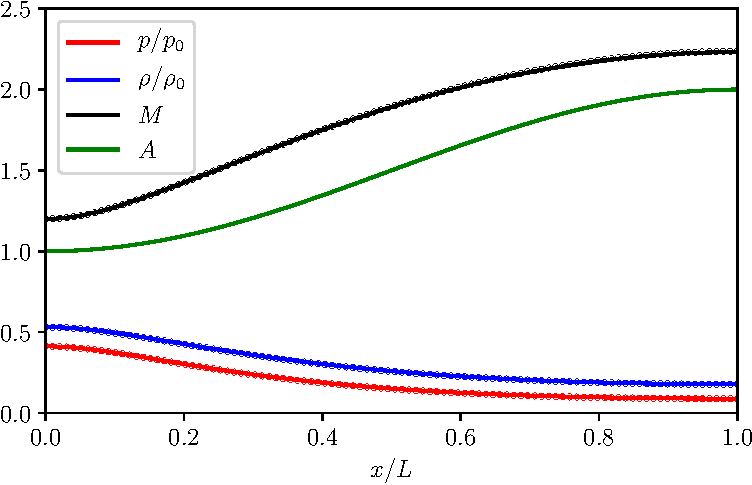
\includegraphics[width=84mm]{isentropicNozzle}
	\caption{\label{FIG_IN} Comparison of the numerical ($\circ$) and analytical ($-$) solutions to a steady isentropic flow with variable-area nozzle geometry. The grid resolution is $n_x=100$.}
\end{figure}
\subsection{Laminar Flame}
The implementation of the diffusive fluxes in \stnshk\ is verified using a premixed laminar flame test case. \cantera's built-in steady eigenvalue solution for a premixed laminar flame is employed for comparison. A stoichiometric hydrogen/air flame at the initial conditions $T$=300 K and $p$=1 bar is simulated using the detailed mechanism due to Hong~\emph{et al.}~\cite{HONG_DAVIDSON_HANSON_CF11}. It is shown in Fig.~\ref{FIG_LF} that the flame structure of the \stnshk\ solution matches that of the \cantera\ solution to good accuracy with 5 cells across the flame. Hence, the implemented diffusive fluxes and reaction chemistry in \stnshk\ are verified to reproduce the chemico-diffusive coupling inherent in a premixed laminar flame. 
\begin{figure}[!ht!]
	\centering
	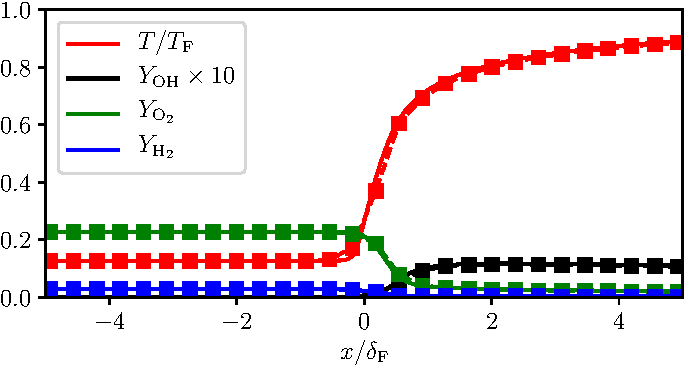
\includegraphics[width=84mm]{laminarFlame.pdf}
	\caption{\label{FIG_LF} Comparison of the \stnshk\ (-$\square$-) and \cantera ($--$) solutions to a steady, premixed laminar flame. The flame thickness, $\delta_\mathrm{f}=368\mu$m, is defined as twice the inverse of the logarithmic temperature gradient. }
\end{figure}
\subsection{Zeldovich-von Neumann-D\"oring Detonation}

The Zeldovich-von Neumann-D\"oring (ZND) structure of a laminar detonation  is used for verification o fthe reacting flow model. A comparison of \stnshk\ to the solution of the ZND equations is given in Fig.~\ref{FIG_ZND}. The solution to the ZND equations is found using a stiff ODE solver, and details about the solution may be found in Lee~\cite{LEE_BOOK2008}. The hydrogen-oxygen mechanism due to Burke~\emph{et al.}~\cite{BURKE_CHAOS_JU_DRYER_KLIPPENSTEIN_IJCK20112} is employed for the chemical model. The mixture consists of stoichiometric H$_2$-Air with an initial pressure of $0.1$ bar and temperature of 300 K. The \stnshk\ solution is initialized from a uniform von Neumann state with the inlet condition at the von Neumann state and a constant back-pressure at the CJ pressure. The initial von Neumann state corresponds to $[\rho_\mathrm{vN},u_\mathrm{vN},p_\mathrm{vN}]=[0.441\ \mathrm{kg/m^3}, 	369\ \mathrm{m/s},25.9\ \mathrm{bar}]$ for the mixture. The grid is resolved to $l_\mathrm{ind}/\Delta x=185$, where $l_\mathrm{ind}:=|\arg\max_{x}Y_\mathrm{OH}(x)|$. 

 The velocity is found to be slightly overpredicted by 1.65\% at $x/l_\mathrm{ind}=-1$; this may be due to the finite domain of the one-dimensional \stnshk\ simulation. However, the ability of \stnshk\ to model laminar detonation chemistry is shown to be quite good overall. Particularly, pressure, density, and mass fractions shown do not deviate significantly from the analytical solution. Hence, \stnshk\ is demonstrated to perform reasonably well in capturing high-speed combustion chemistry in the absence of significant diffusive effects.

\begin{figure}[!ht!]
	\centering
	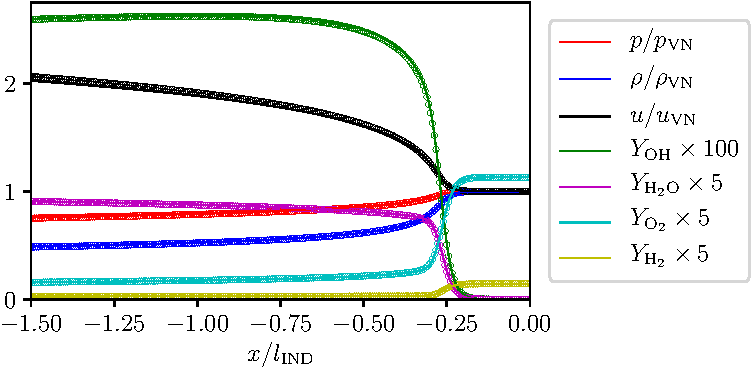
\includegraphics[width=84mm]{ZNDDetonation}
	\caption{\label{FIG_ZND} Comparison of numerical ($\circ$) and analytical ($-$) solutions to a laminar ZND detonation. The grid resolution is $l_\mathrm{ind}/\Delta x=185$. The mixture is stoichiometric H$_2$-Air with an initial state of $p_0=0.1$ bar and $T_0=300$ K.} 
\end{figure}

\subsection{Validation Cases}

Of primary interest in this model is the prediction of the temporal pressure rise behind the reflected shock as reported by Pang~\emph{et al.}~\cite{PANG_DAVIDSON_HANSON_PCI32}. The temporal pressure rise increases the reaction rate of the test mixture above that predicted by homogeneous reactor models for conventional shock tubes. Additionally, a rise in pressure in the test section implies a corresponding rise in temperature, which further accelerates the reaction rate by increasing the value of the kinetic rate coefficients. Homogeneous reactor models, which incorporate an experimental pressure trace, have been shown to produce reasonable correspondence to experimental data~\cite{PANG_DAVIDSON_HANSON_PCI32}; however, the utility of these models in supporting the design of experiments is limited since they do not model the underlying physical mechanisms that are responsible for producing the temporal pressure rise. Hence, the ability of \stnshk\ to capture this boundary layer effect using the source terms given in Eq.~\ref{EQ_BLSRC} is examined. To this end, \stnshk\ is compared to experimental data from the Stanford Aerosol Shock Tube (AST)~\cite{CAMPBELL_THESIS}. The AST  has a driven section diameter and length of 11.4 cm and 9.73 m, respectively. The length of the driver section is constant at 3.60~m. 

A case matrix detailing the differences between the different \stnshk\ calculations is given in Table~\ref{TABLE_CASE}. The capabilities of \stnshk\ to model shock tube experiments with boundary layer effects are validated through four cases with increasing complexity:
\begin{enumerate}
	\item Examine the baseline capabilities of \stnshk\ to produce an experimental pressure trace in a homogeneous mixture without area variation.
	\item Examine a homogeneous mixture with a sharp area variation between the driver and driven sections.
	\item Examine the use of a driver section insert.
	\item Examine tailoring via disparate driver section and driven section mixtures with area variation via a driver insert. 
\end{enumerate}
A driver section insert is utilized for two of the test cases, and the geometries are shown in Fig.~\ref{FIG_DIVG}. All cases are initialized as a Riemann problem with the pressures and temperatures given in Table~\ref{TABLE_CASE}. The shock tube is assumed to initially be in thermal equilibrium (i.e., $T_1=T_4=T$) with zero gas velocity, and the side wall temperature used for the boundary layer model is set to the initial equilibrium temperature. The end wall boundary conditions are adiabatic and reflecting. Discontinuities in area are smoothed across 10 cells to reduce numerical stiffness, and $n_x = 1000$ cells are utilized in all simulations.
\begin{figure}[!h!]
	\centering
	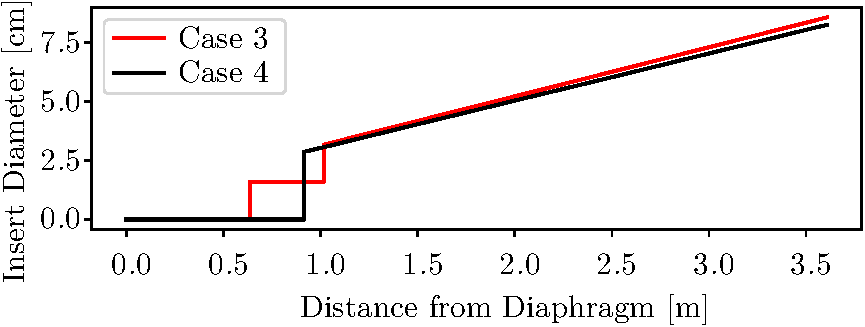
\includegraphics[width=84mm]{driverInsertValidation_geometries}
	\caption{\label{FIG_DIVG} Driver section insert geometries used for validation.} 
\end{figure}
\begin{table}[!ht!]
	\centering
	\footnotesize
	\resizebox{120mm}{!}{
		\begin{tabular}{|c|c|c|c|c|c|c|c|c|}
			\hline
			ID 		& $D_4$ [cm]& Insert   	& $p_4$	[kPa]	& $\Xvec_4$			& $p_1$	[kPa] & $\Xvec_1$ & 	$T$ [K]	 \\ 
			\hline
			1		& 11.4		& N			&  233 			& 100\% \ce{N2}  & 2.03   	&  100\% \ce{N2}	& 292.05		\\ 
			2		& 17.8		& N			&  211 			& 100\% \ce{N2}  & 2.03   	&  100\% \ce{N2}	& 291.75		\\ 
			3		& 11.4		& Y			&  247 			& 100\% \ce{N2}  & 2.00   	&  100\% \ce{N2}	& 292.25		\\ 
			4		& 11.4		& Y			&  509 			& 75\% \ce{N2}, 25\% \ce{He}  & 52.0   	&  79\% \ce{Ar}, 21\% \ce{O2}	& 292.05 		\\ 
			\hline
		\end{tabular}
	}
	\caption{\label{TABLE_CASE} Summary of configurations for \stnshk\ validation calculations.}
\end{table}

As shown in Fig.~\ref{FIG_VAL}, \stnshk\ reproduces experimental data to good accuracy. In particular, the rise in the test pressure is shown to be well replicated for the case with the boundary layer model when compared to the case without the boundary layer model. Additionally, without the boundary layer model, the initial test pressure is over-predicted. Furthermore, sharp jumps are apparent in Cases 1-3 without the boundary layer model, which are due to the interaction of the reflected shock with the contact discontinuity and the subsequent reverberations.  

The results in Fig.~\ref{FIG_VAL} indicate \stnshk's utility in the design of experiments in predicting cases with a significant influence of the boundary layer. Hence, \stnshk\ is shown to be capable of modeling effects of a driver insert, the boundary layer, and driver/driven gas composition on the one-dimensional gas dynamics.   


\begin{figure}[!h!]
	\centering
	\subfigure[\label{FIG_VAL_CONSTANT_AREA}Case 1]{
		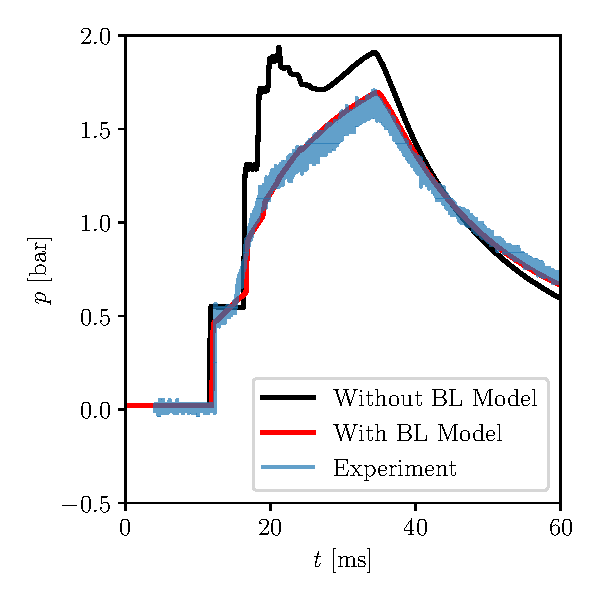
\includegraphics[width=0.475\textwidth]{testCase_constantArea}}
	\subfigure[\label{FIG_VAL_STEP_AREA}Case 2]{
		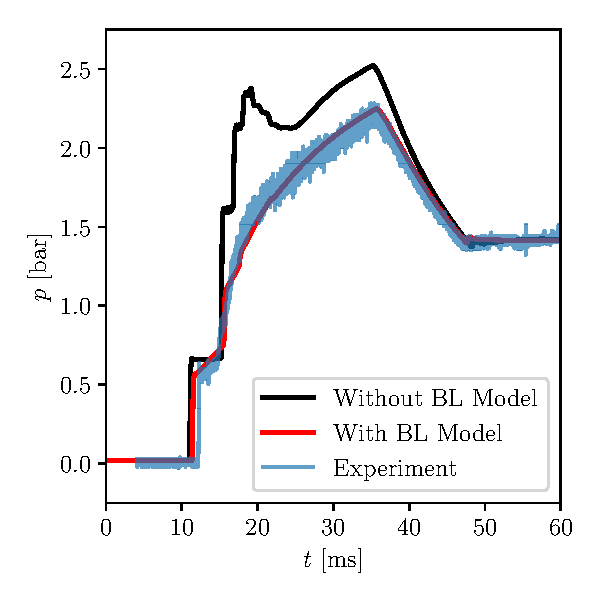
\includegraphics[width=0.475\textwidth]{testCase_stepChange}}
	\end{figure}
	\begin{figure}[!h!]
		\centering
	\subfigure[\label{FIG_VAL_DRIVER_INSERT}Case 3]{
		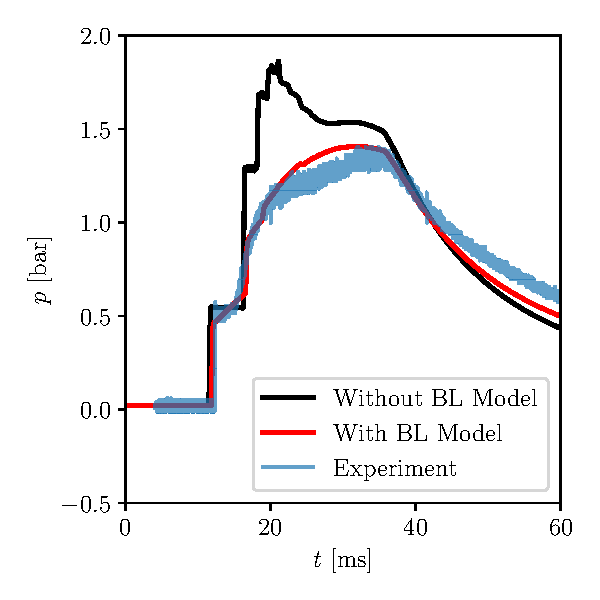
\includegraphics[width=0.475\textwidth]{testCase_driverInsert}}
	\subfigure[\label{FIG_VAL_DISSIMILAR_GAS}Case 4]{
		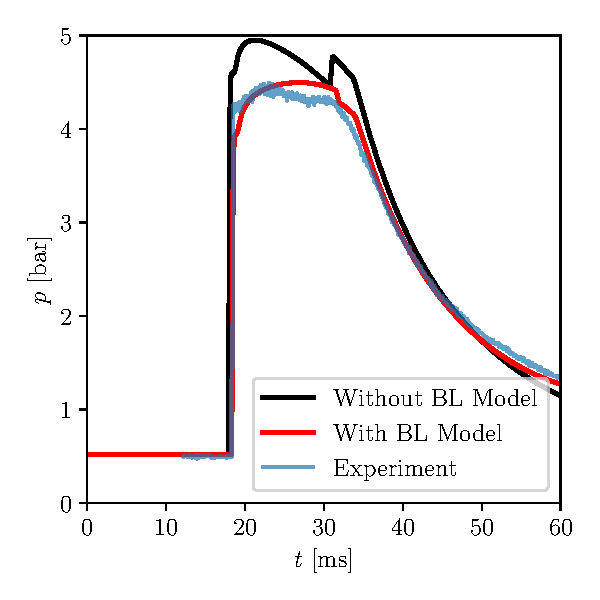
\includegraphics[width=0.475\textwidth]{testCase_dissimilarGas}}
	\caption{\label{FIG_VAL} Validation results for the test cases described in Table~\ref{TABLE_CASE}. The pressure trace is taken at the end wall of the shock tube. One thousand cells were utilized for these solutions.}
\end{figure}	
%%%%%%%%%%%%%%%%%%%%%%%%%%%%%%%%%%%%%%%%%%%%%%%%%%%%%%%%%%%%%%%%%%%%%%%%%%%%%%%%%%%%%%%%%%%%%%%%%%%%%%%%%%%%%%%%%%%%
\subsubsection{Sensitivity of the Boundary Layer Model}
Since the boundary layer model discussed in Sec.~\ref{SEC_MODEL} relies on empirical correlations for the skin friction coefficient and the Nusselt number, a degree of variation in the model performance can be expected due to the uncertainty in the model parameters. Furthermore, tuning these model parameters may be appropriate to account for the unique design features of a particular shock tube (e.g, non-circular cross-section and bends). Hence, the sensitivity of \stnshk\ to the skin friction and heat transfer terms is examined by separately perturbing these terms by a multiplicative factor.  Furthermore, since small diameter shock tubes are of interest due to their capability for providing a large sample size of chemical kinetic measurements~\cite{TRANTER_LYNCH_RSI2013}, the sensitivity of the gas dynamics to a reduction in the shock tube diameter is investigated.

\begin{figure}[!h!]
	\centering
	\subfigure[\label{FIG_SENSANAL_PR}Pressure Rise]{
		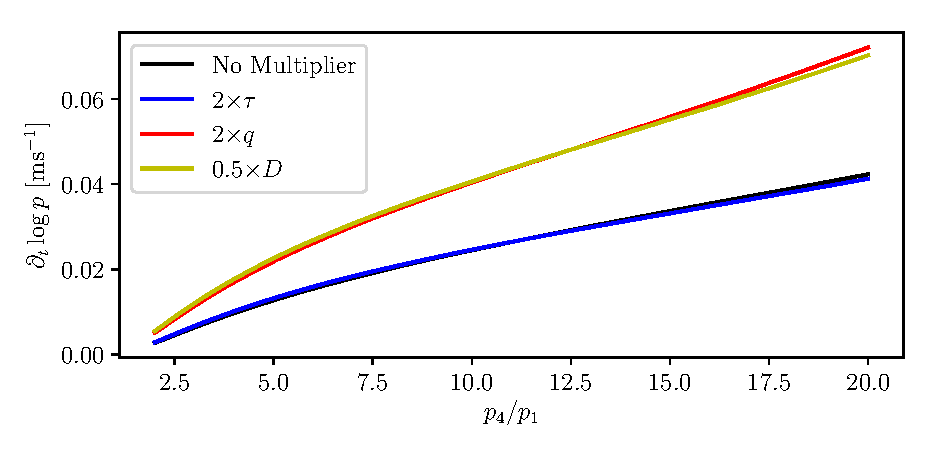
\includegraphics[width=80mm]{sensitivity_pressureRise}}
	\subfigure[\label{FIG_SENSANAL_P5}Test Pressure]{
		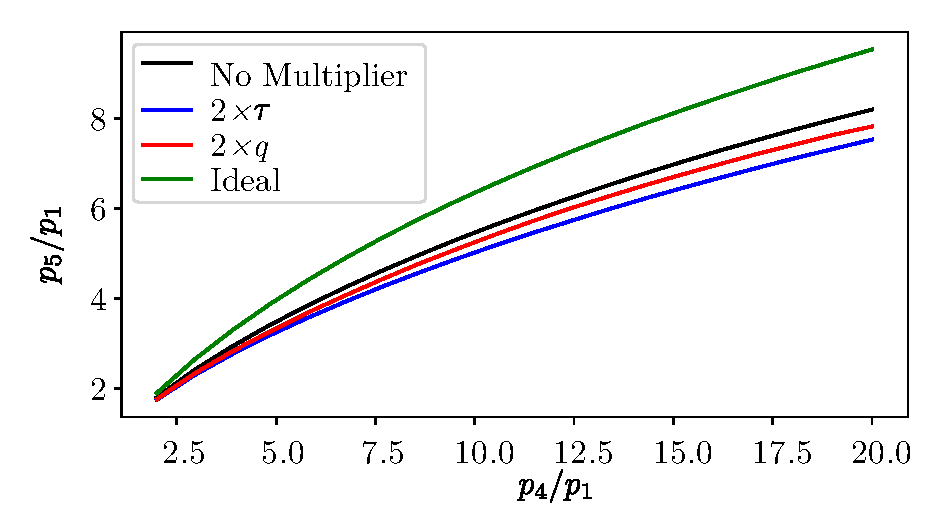
\includegraphics[width=80mm]{sensitivity_testPressure}}
	\subfigure[\label{FIG_SENSANAL_SA}Incident Shock Attenuation]{
		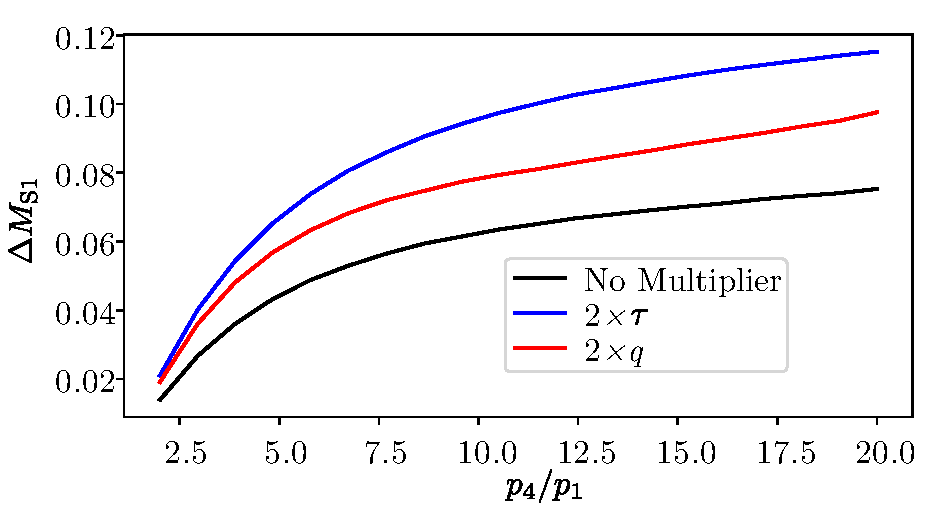
\includegraphics[width=80mm]{sensitivity_MachNumber}}
	\caption{\label{FIG_SENSANAL} Sensitivity of the boundary layer model to adjustments in the skin friction, heat transfer, and shock tube diameter.}
\end{figure}

The results of these calculations are shown in Fig.~\ref{FIG_SENSANAL} for a range of initial pressure ratios with a driven section pressure of $p_1=1$ bar. The initial temperature and velocity are set to 300 K and 0 m/s, respectively, throughout the domain. Argon is utilized for the driver and driven gas in a shock tube with a uniform cross-section with a baseline diameter of 5 cm, a driver length of 3 m, and a driven length of 5 m; 500 cells are used to compute the quantities shown. The ideal quantities are computed using normal shock relations, which do not include the effect of the boundary layer. Incident shock Mach number attenuation is computed using the difference between the ideal incident Mach number and that taken from \stnshk.

It is evident from Fig.~\ref{FIG_SENSANAL_PR} that the predicted pressure rise shows a substantial sensitivity to the heat transfer while it is relatively insensitive to the skin friction coefficient. The increase in the test pressure is primarily due to the convective boundary layer in front of the reflected shock; that is, pressure disturbances due to heat loss transmit through the reflected shock into the test gas. Heat loss to the walls occurs in the quiescent post-shock test gas; however, this effect tends to reduce the test pressure, and hence, it is unlikely to control the dynamics of the test pressure. The tendency for a nearly quiescent gas to loose pressure can be easily shown with simple thermodynamic relations and is a well-known phenomena in rapid compression machine experiments~\cite{LEE_HOCHGREB_CF1998,IHME_CF2012}. Interestingly, this model implies that a reduction in the sidewall heat transfer could be an effective means of decreasing the rise in test pressure.


An increase in the skin friction yields a much more potent effect on the predicted test pressure than the heat transfer as demonstrated in Fig.~\ref{FIG_SENSANAL_P5}. Additionally, the incident shock attenuation is shown to increase with increasing skin friction and heat transfer.

As expected, the reduction in the shock tube diameter significantly increases the rate of the rise in test pressure, reduces the test pressure, and increases the attenuation of the incident shock wave. For the rate of the rise in the test pressure, reducing the diameter by a factor of two is shown to have a nearly equivalent effect as increasing the heat transfer by a factor of two. This is due to the boundary layer source term in the energy equation being covariant and contravariant with the heat transfer and the tube diameter, respectively. 


%%%%%%%%%%%%%%%%%%%%%%%%%%%%%%%%%%%%%%%%%%%%%%%%%%%%%%%%%%%%%%%%%%%%%%%%%%%%%%%%%%%%%%%%%%%%%%%%%%%%%%%%%%%%%%%%%%%%
\section{Applications}\label{SEC_APPLICATIONS}
%%%%%%%%%%%%%%%%%%%%%%%%%%%%%%%%%%%%%%%%%%%%%%%%%%%%%%%%%%%%%%%%%%%%%%%%%%%%%%%%%%%%%%%%%%%%%%%%%%%%%%%%%%%%%%%%%%%%
\subsection{Simulation of Experiment with an Uncertain Chemical Kinetic Model}
From Sec.~\ref{SEC_VV}, \stnshk\ is demonstrated to replicate key experimental observations including the temporal pressure rise in the test section and the attenuation of the incident shock wave. Following these validation tests, a simulated experiment is performed to quantify the performance of a chemical mechanism to predict a shock tube experiment. 

Towards this end, the mechanism of Hong~\emph{et al.}~\cite{HONG_DAVIDSON_HANSON_CF11} is utilized to simulate the experiment of Pang~\emph{et al.}~\cite{PANG_DAVIDSON_HANSON_PCI32}. One thousand Monte Carlo samples from the provided uncertainty bounds of Hong~\emph{et al.} are propagated with \stnshk, and the results are depicted in Fig.~\ref{FIG_PTUQ}. As with previous results, \stnshk\ shows good agreement with the experiment with respect to the post-reflected-shock pressure rise.  However, \stnshk\ is shown to under-predict the peak pressure compared to the experiment. This is likely due to multi-dimensional effects such as blast wave reflection being present in the experiment. The \stnshk\ simulation only proceeded to the extent of the experimental data, which is 7.6 ms after shock reflection; however, only 27\% of the \stnshk\ cases ignited by this time indicating that the mechanism over-predicts ignition delay with respect to the experiment and that the temporal increase in the test pressure assists in igniting the mixture.
\begin{figure}[!ht!]
	\centering
	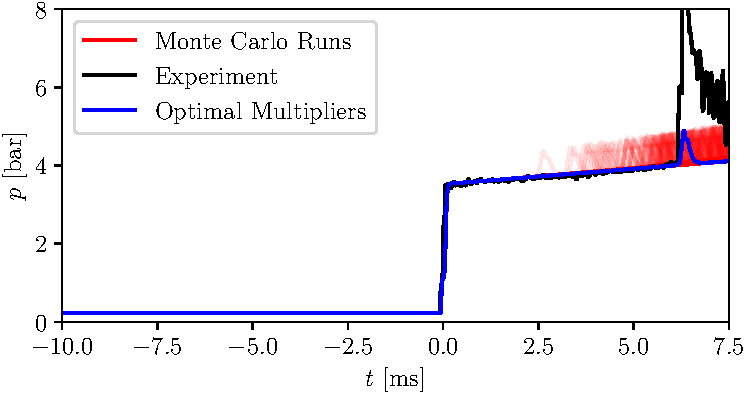
\includegraphics[width=84mm]{pressureTraceUQ}
	\caption{\label{FIG_PTUQ} Comparison of Monte Carlo runs of \stnshk\ to the experiment of Pang~\emph{et al.}~\cite{PANG_DAVIDSON_HANSON_PCI32} using the chemical mechanism of Hong~\emph{et al.}~\cite{HONG_DAVIDSON_HANSON_CF11}. The mixture is stoichiometric hydrogen/oxygen with 94\% dilution and $T_5=940$ K, $p_5=$3.5 bars.} 
\end{figure}
The optimal multipliers curve, shown in Fig.~\ref{FIG_PTUQ}, denotes the set of forward rate coefficient multipliers that yield the best agreement with the experiment. This is found using a Gaussian Process Regression surrogate model~\cite{SANTER_BOOK} in conjunction with a constrained optimization, which minimizes the variance of the surrogate model subject to the predicted ignition delay being equal to the experimental value. The normalized forward rate coefficient ($k_\mathrm{f,opt}/k_\mathrm{f}$) and their sensitivities about the optimal point are given in Table~\ref{TABLE_MULTS}. Since the standard rate coefficient ($k_\mathrm{f}$) for the mechanism over-predicts the ignition delay for the experiment under examination, a faster hydrogen radical and oxygen radical branching reaction (1) and a slower hydrogen peroxide termination reaction in the argon bath (2a) are found by the optimizer -- both of which serve to reduce the ignition time. Other reactions such as the water formation and oxygen radical propagation reaction (6) demonstrate a large change in the forward rate multiplier, but the ignition time is relatively insensitive to their alteration. 
\begin{table}[!t!]
	\centering
	\footnotesize
	\resizebox{120mm}{!}{
		\begin{tabular}{|c|c|c|c|}
			\hline
			No. & Rxn. & $k_\mathrm{f,opt}/k_\mathrm{f}$ & $k_\mathrm{f}(\p\tau_\mathrm{ign}/\p k_\mathrm{f,opt})$ [ms] 	 	 \\ 
			\hline
			1 & H + \ce{O2} $\longleftrightarrow$ O + OH 			& 1.09 & -1.31e+01 \\
			2a & H + \ce{O2} (+Ar) $\longleftrightarrow$ \ce{HO2} (+Ar) 	& 0.83 & 1.31e+01 \\
			2b & H + \ce{O2} (+\ce{H2O}) $\longleftrightarrow$ \ce{HO2} (+\ce{H2O})& 0.98 & 1.80e-01 \\
			2c & H + \ce{O2} (+\ce{O2)} $\longleftrightarrow$ \ce{HO2} (+\ce{O2}) 	& 0.99 & 5.13e-01 \\
			2d & H + \ce{O2} (+M) $\longleftrightarrow$ \ce{HO2} (+M) 	& 0.92 & 2.76e+00 \\
			3 & \ce{H2O2} (+M) $\longleftrightarrow$ 2 OH (+M) 	& 0.97 & -5.31e-02 \\
			4 & \ce{H2O2} + OH $\longleftrightarrow$ \ce{H2O} + \ce{HO2} 	& 0.98 & 4.66e-02 \\
			5 & \ce{HO2} + \ce{OH} $\longleftrightarrow$ \ce{H2O} + \ce{O2} 		& 1.06 & 7.87e-02 \\
			8 & 2 OH $\longleftrightarrow$ \ce{H2O} + O 			& 1.13 & 8.90e-02\\
			\hline
		\end{tabular}
	}
	\caption{\label{TABLE_MULTS} Forward rate coefficients and sensitivities found to correspond best to the experiment. Only reactions with reported uncertainties are utilized. Reaction numbering corresponds to that of Hong~\emph{et al.} with lettering added to distinguish third-body species.}
\end{table}

%%%%%%%%%%%%%%%%%%%%%%%%%%%%%%%%%%%%%%%%%%%%%%%%%%%%%%%%%%%%%%%%%%%%%%%%%%%%%%%%%%%%%%%%%%%%%%%%%%%%%%%%%%%%%%%%%%%%
\subsection{Optimization of Driver Inserts}\label{SUBSEC_OPT}
As noted in preceding sections, the formation of the boundary layer trailing the incident shock yields a temporal increase in the pressure of the test gas. Driver inserts are a method to counter-act the increase in the test pressure by reflecting a portion of the expansion fan before it reaches the driver end wall. 

Hong~\emph{et al.}~\cite{HONG_PANG_VASU_DAVIDSON_HANSON_SW2009} developed a method for designing conical inserts to reduce the unsteadiness of the test pressure. Key to the design of the inserts is the variable-area theory of Alpher and White~\cite{ALPHER_JFM58}, which quantifies the effect of an area change in the driver section on the test pressure. Furthermore, Hong~\emph{et al.} assumed that the effects of the boundary layer and the area change can approximately be superposed to yield a steady test pressure. However, the process to design the correct driver inserts is extensive and often laborious. Furthermore, the analytical model suffers from the assumption that the area change interacts linearly with the displacement due to the boundary layer. Hence, it is proposed that \stnshk\ may be utilized in conjunction with a global optimization algorithm to discover an optimal experimental design. 

\begin{figure}[!h!]
	\centering
	\subfigure[\label{FIG_HONG_P} Pressure trace]{
		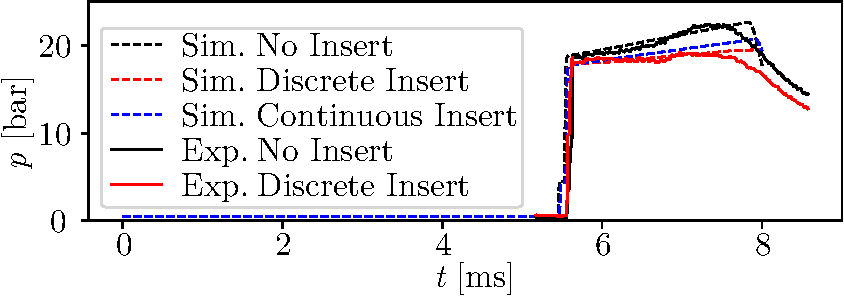
\includegraphics[width=80mm]{driverInsert_traces}}
	\subfigure[\label{FIG_HONG_A} Geometry]{
		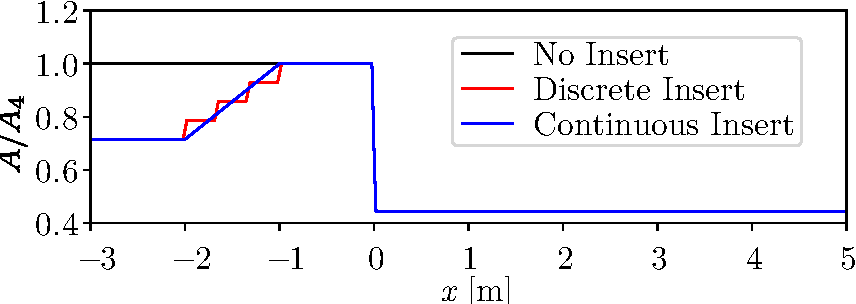
\includegraphics[width=80mm]{driverInsert_geometries}}
	\caption{\label{FIG_HONG} Comparison of the experimental pressure traces with \stnshk\ calculations and corresponding effective geometry of the shock tubes.}
\end{figure}

First, \stnshk\ is employed to simulate the configuration of Hong~\emph{et al.} to ensure that reasonable replications of the experimental pressure traces are obtained for the base geometry without an insert and the optimal geometry with an insert. The pressure traces reported by Hong~\emph{et al.} are compared to the output of \stnshk\ in Fig.~\ref{FIG_HONG}. For these simulations, the driver pressure is $p_4=12$ bar and the driven pressure is $p_1=0.48$ bar. The driver gas is pure helium, while the driven gas is argon. The initial temperature is taken to be 283 K. The experimental pressure traces are obtained from the Stanford High Pressure Shock Tube~\cite{HONG_PANG_VASU_DAVIDSON_HANSON_SW2009}. The simulations utilize 500 cells and the solution is obtained within a minute on a laptop.  

The analytical model of Hong~\emph{et al.} assumes a linear decrement in the driver area, which yields a parabolic end-section for the insert. However, to ease the production of the inserts, they are coarsely discretized; a depiction of the continuous and discretized geometries is shown in Fig.~\ref{FIG_HONG_A}. Interestingly, the simulation shows that the discretization of the geometry reduces the rise in test pressure compared to that for the  continuous geometry. Since the discrete geometry is used in the experiment, it is unsurprising that it is a better match to the test pressure trace than the analytical geometry. Additionally, the experiment shows a small bump in the experimental pressure trace that is not present in the \stnshk\ simulation. This is likely due to interactions of the contact surface with the reflected shock and the end wall.
 
 While \stnshk\ can effectively model material interfaces by utilizing the double flux model discussed in Sec.~\ref{SEC_MODEL}, a quasi-1D solver is incapable of modeling complex mixing processes occurring during the rupturing of the diaphragm. Improved agreement could possibly be found by utilizing a smoothed interface between the driver and driven gasses rather than a step function to better approach the physics of the initial incident shock formation. Additionally, the shock tube may be simulated with a semi-infinite domain with only the test section by utilizing a supersonic inflow at state ($p_2, T_2$) as is done in high-fidelity simulations~\cite{GROGAN_PCI2015}; this would help isolate the effect of the contact surface for a particular experimental condition.

 Overall, it is surmised that \stnshk\ does a reasonable job at reproducing the experimental pressure traces -- particularly during the test time (about 5.5--7.5 ms). Hence, confidence is gained with respect to \stnshk's ability to reproduce the results of non-optimal and optimal configurations, and a optimization procedure may be employed with assurance that additional designs sampled from the parameter space for this experiment will likely correspond to realistic gas dynamics. 

We proceed by employing \stnshk\ for optimizing the geometry of the driver insert for the same operating conditions. This optimization problem is defined in the following fashion:
\begin{mini}|l|
	{\boldsymbol\theta}{\left(\frac{\partial \log p(x,\tau;\boldsymbol \theta)}{\partial \tau}\right)^2+\lambda\left(\frac{\bar p(x,\tau;\boldsymbol \theta)}{p_5}-1\right)^2}{}{}
	\addConstraint{\boldsymbol \theta}{= [L,D,\alpha]^\top}{}
	\addConstraint{x}{= x_\mathrm{ew}}{}
	\addConstraint{\tau}{= \frac{t-\tau_\mathrm{shk}}{\tau_\mathrm{test}}}{}
	\addConstraint{0}{\le \tau }\le{1}
	\addConstraint{0}{\le L/L_\mathrm{driver} }\le{1}
	\addConstraint{0}{\le D/D_\mathrm{driver} }\le{1}
	\addConstraint{0}{\le \alpha }\le{1}\ ,
	\label{EQ_OPT}
\end{mini}
where the test time is given by $\tau_\mathrm{test}$ and is defined as the interval between the time of shock reflection ($\tau_\mathrm{shk}$) and the arrival of the expansion fan or the contact surface (with the latter being germane for non-tailored experiments); the end wall probe location for the \stnshk\ simulation is denoted by $x_\mathrm{ew}$. The trade-off parameter, $\lambda$, allows the modeler to decide which objective is to be emphasized in the multi-objective problem. The target test pressure is given by $p_5$, and the bar operater (i.e., $\bar p$) indicates that the pressure at the end wall is temporally averaged over the test time. The length and diameter of the driver section are denoted by $L_\mathrm{driver}$ and $D_\mathrm{driver}$, respectively.

The first objective acts to reduce the pressure rise in the simulated pressure trace while the secondary objective acts to yield a pressure trace that is near the expected test condition. Furthermore, if one defines $\boldsymbol\chi=\left[\p_\tau\log p,\sqrt{\lambda}\left(\bar p/p_5-1\right)\right]^\top$, then the objective function is simply given by $\|\boldsymbol{\chi}\|_2^2\in[0,\infty)$, and it is clear that the optimal set is given by $\Theta=\{\boldsymbol{\theta}\in\mathcal D\ |\ \|\boldsymbol\chi\|_2^2=0\}$, where $\mathcal{D}$ is the design space of the optimization problem (assuming $\boldsymbol\chi = 0$ is feasible). The choice of the norm for the optimization problem is an additional hyperparameter; however, the Euclidean norm is chosen ab initio due to its smoothness properties.

The design parameters (i.e., $L,\ D$, and $\alpha$) are the length of the insert, the diameter of the insert, and the portion of the insert for which the area is constant; the insert geometry is modeled after the analytical geometry given by Hong~\emph{et al.} and is similar to the continuous insert geometry shown in Fig.~\ref{FIG_HONG_A}. Note that the design parameters are constant for a given \stnshk\ run, and the shock tube geometry other than the insert is constant for all runs.

The primary goal in solving the optimization problem, given by Eq.~\ref{EQ_OPT}, is to find an optimal solution in as few \stnshk\ runs as necessary. Since the objective function requires the numerical solution of a coupled set of non-linear, partial differential equations with discontinuous solutions, few theoretical guarantees may be made about the solution surface (e.g., convexity). Traditional optimization routines such as gradient descent and Newton iterations can find local optima, but often do not yield a satisfactory design. Furthermore, exhaustive sampling of the parameter space would be prohibitively expensive for the code's intended use. For example, a 100$^3$ grid of the parameter space would require $\mathcal{O}(10^3)$ CPU-hrs to solve; while this expense is certainly feasible if high-performance computing resources are available, it is not a viable option given only a desktop or laptop computer (approximately a month of computing). Hence, a global sampling method is employed, which uses a Gaussian Process (GP) as a surrogate model to determine the optimal points in the parameter space to sample~\cite{SANTER_BOOK,RASMUSSEN_BOOK}. 

Gaussian Processes are a popular model surrogate for the output of computer simulations since they interpolate between known outputs (unlike standard parametric regressors), and they provide a probabilistic interpretation of the interpolated points (unlike non-parametric models such as splines). The latter property can be expanded into a useful metric to decide where to sample in a global search. More details about the use of Gaussian Processes in the global optimization procedure are given in ref.~\cite{GROGAN_THESIS18}.

The Gaussian Process sampling method is applied to the driver insert optimization problem detailed by Eq.~\ref{EQ_OPT}, and the resulting pressure traces and optimized geometry are shown in Fig.~\ref{FIG_OPT}. The initial configuration is that of Hong~\emph{et al.}~\cite{HONG_PANG_VASU_DAVIDSON_HANSON_SW2009} with the matching \stnshk\ results of this study shown in Fig.~\ref{FIG_HONG}. A comparative table of results is reported in Table~\ref{TABLE_OPT}. The pressure rise for a given pressure trace is approximated by first extracting the test region ($t\in[\tau_\mathrm{shk},\tau_\mathrm{shk}+\tau_\mathrm{test}]$) and then finding the logarithmic difference in the pressure over the time:
\begin{equation}\label{EQ_PR}
\left . \frac{\p \log p}{\p t}\right |_{x=x_\mathrm{ew}}\approx\frac{1}{\tau_\mathrm{shk}}\log\left (\frac{ p(x_\mathrm{ew},\tau_\mathrm{shk}+\tau_\mathrm{test})}{p(x_\mathrm{ew},\tau_\mathrm{shk})}\right)\ .
\end{equation}
The pressure rise computation is tantamount to determining the mean pressure rise over the test interval. 

The optimization routine requires 30 iterations to determine an optimium within tolerance and takes approximately 40 seconds to compute on a laptop. During optimization, a relatively coarse mesh of 200 cells was found to be sufficient to resolve the objective function. However, it is noted that additional uncertainty with respect to mesh convergence or other known bias can be formally incorporated in the GP regressor; this would yield a stochastic optimization problem rather than the deterministic problem currently examined.   

\begin{figure}[!ht!]
	\centering
	\subfigure[\label{FIG_OPT_P} Pressure trace]{
		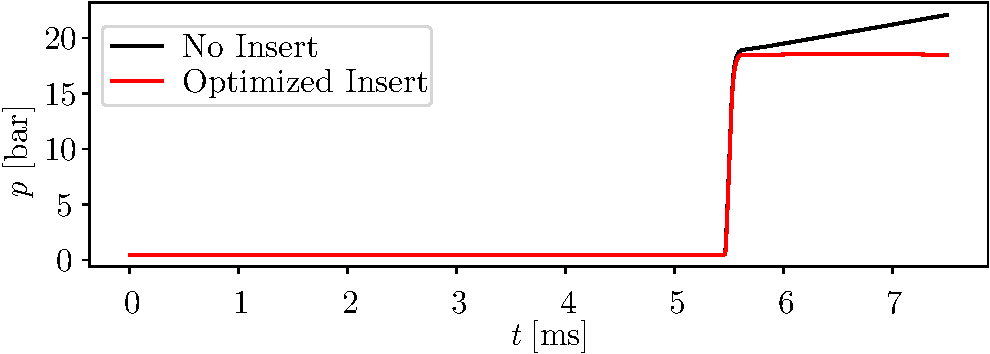
\includegraphics[width=84mm]{driverInsert_pOpt}}
	\subfigure[\label{FIG_OPT_A} Geometry]{
		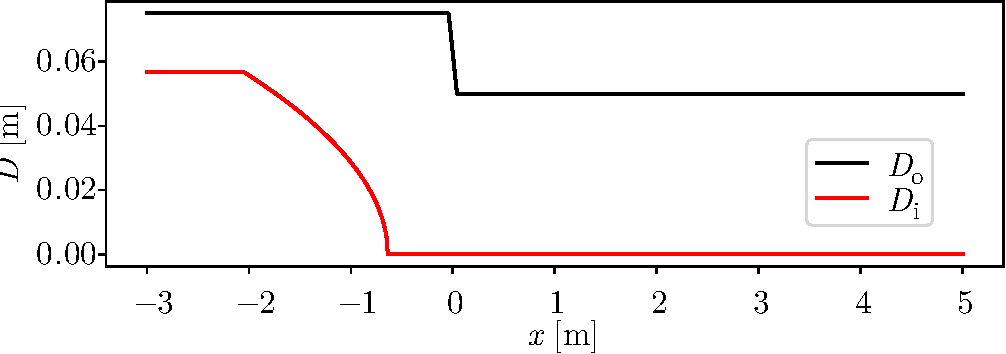
\includegraphics[width=84mm]{driverInsert_DOpt}}
	\caption{\label{FIG_OPT} Results of the driver insert optimization detailed in Eq.~\ref{EQ_OPT}. The driver pressure is $p_4=12$ bar and the driven pressure is $p_1=0.48$ bar. The driver gas is pure helium, while the driven gas is argon. The initial temperature is taken to be 283 K.}
\end{figure}

As desired, the pressure trace for the optimized insert is shown to be relatively flat in Fig.~\ref{FIG_OPT_P}. However, as demonstrated by Fig.~\ref{FIG_HONG_P}, the discretization of the insert may yield results differing from the continuous geometry used for the optimization; this discrepancy could be rectified by inserting a bias in the pressure rise measurement or by expanding the parameter space to include discrete geometries. Additionally, a comparison of the $x$-$t$ diagrams for the pressure of the shock tube is given for both cases in Fig.~\ref{FIG_XTOPT}. Primarily, the test region is shown to have a relative constant pressure at the end wall ($x=5$ m) for the optimized insert case. Furthermore, the pressure in the driver section behind the expansion fan is shown to be decreasing in the optimized insert case due to the action of the variable geometry. Also, an abrupt difference in pressure is observed near the change in the outer geometry of the shock tube ($x=0$). This is due to the flow being subsonic near the discontinuity, which leads to a decrease in pressure per the contraction of the flow. Additionally, a slight dip in pressure is shown trailing the expansion fan; this is due to the necessity to smooth the jump in driver-side and driven-side areas for numerical stability; however, end wall pressure traces are found to be insensitive to resolution.

\begin{figure}[!ht!]
	\centering
	\subfigure[\label{FIG_XTOPT_INS}Without Insert]{
		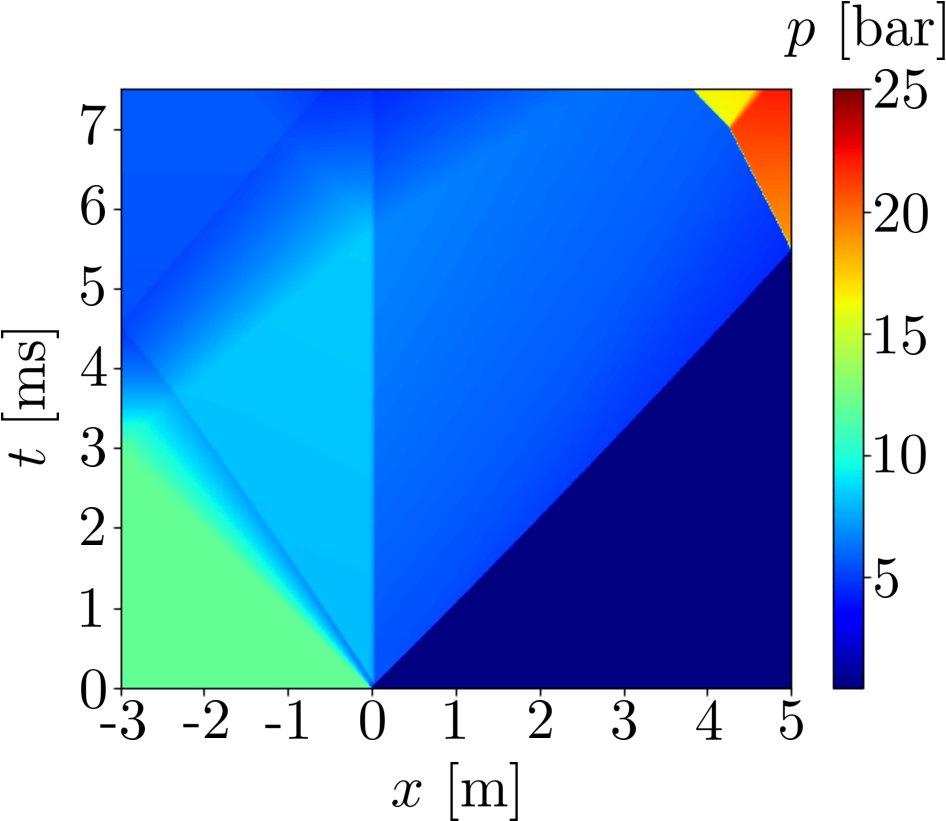
\includegraphics[width=0.475\textwidth]{driverInsert_XTNoIns.pdf}}
	\subfigure[\label{FIG_XTOPT_NOINS} Optimized Insert]{
		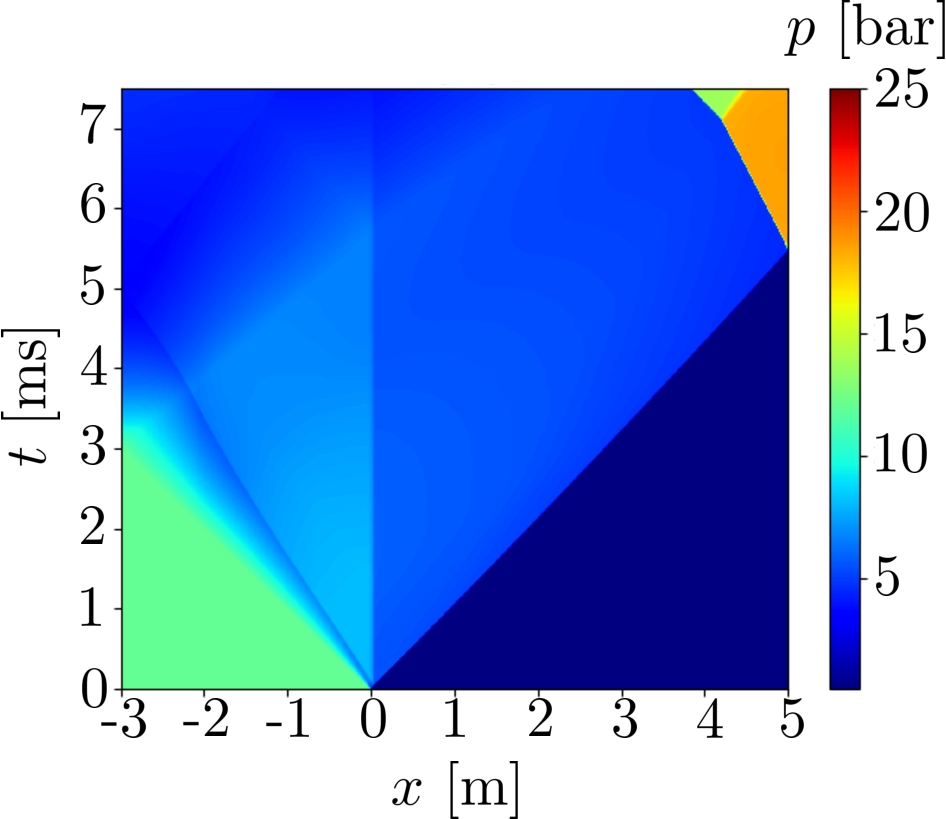
\includegraphics[width=0.475\textwidth]{driverInsert_XTIns.pdf}}
	\caption{\label{FIG_XTOPT}$x$-$t$ diagrams of pressure for cases (a) without driver insert and (b) with optimized driver insert cases, given in the last two rows of Table~\ref{TABLE_OPT}. The driver pressure is $p_4=12$ bar and the driven pressure is $p_1=0.48$ bar. The driver gas is pure helium, while the driven gas is argon. The initial temperature is taken to be 283 K. The geometry is shown in Fig.~\ref{FIG_OPT_A}.}
\end{figure}

As given in Table~\ref{TABLE_OPT}, the optimized insert geometry yields the smallest pressure rise in magnitude of the examined configurations; additionally, the test pressure is equivalent to the target pressure of 18.2 bar (the reported experimental value). Hence, the global optization methodology using \stnshk\ and a Gaussian process regressor surrogate model is shown to be an effective and relatively inexpensive way to tailor the gas dynamics of a shock tube experiment.

\begin{table}[!t!]
	\centering
	\footnotesize
	\resizebox{\textwidth}{!}{
		\begin{tabular}{|c|c|c|c|c|c|c|c|}
			\hline
			Data Src.& Ins. Geom. & $L_\mathrm{insert}/L_\mathrm{driver}$	& $D_\mathrm{insert}/D_\mathrm{driver}$				& $\alpha$	& $p_5$ [bar] & $\p \log p/\p t$ [\%/ms]   	 	 \\ 
			\hline
			Exp. & None & -- & -- & -- & 18.5 & 10.3\\
			Sim. & None & -- & -- & -- &  20.8 & 8.3\\
			\hline
			Exp. & Disc. & 0.67 & 0.53 & 0.50 & 18.2 & 2.7\\
			Sim. & Disc. & 0.67 & 0.53 & 0.50 & 18.7 & 4.9\\
			Sim. & Cont. & 0.67 & 0.53 & 0.50 & 19.3 & 6.6\\
			\hline
			Sim. & None & -- & -- & -- & 19.7 & 8.3\\
			Sim. & Opt. & 0.79 & 0.76 & 0.40 & 18.2 & -0.2\\
			\hline
		\end{tabular}
	}
	\caption{\label{TABLE_OPT} Summary table of the configurations for the \stnshk\ driver insert runs. Experimental and simulated pressure rises computed according to Eq.~\ref{EQ_PR}. The shock tube geometry matches that reported by Hong~\emph{et al.}~\cite{HONG_PANG_VASU_DAVIDSON_HANSON_SW2009} for the high pressure shock tube.}
\end{table}
%%%%%%%%%%%%%%%%%%%%%%%%%%%%%%%%%%%%%%%%%%%%%%%%%%%%%%%%%%%%
\section{Conclusions}
A quasi one-dimensional compressible reacting flow solver was developed to simulate shock tube ignition in a computationally inexpensive manner. The solver was constructed in consideration of the relevant physics of a shock tube chemical kinetic study including area variation, disparate gas interfaces, boundary layer development, shock capturing, and reaction chemistry. A fifth-order WENO scheme coupled to a third-order Runge-Kutta time stepping for the advective terms was employed for the discretization, diffusive terms were discretized via central differencing, and Strang splitting with an implicit method was used for the chemical integration. The solver was written in just-in-time compiled object-oriented \python\ to both enhance the portability and to reduce development time. 

\stnshk\ was validated through isentropic nozzle, multi-species Sod's problem, a premixed laminar flame, and laminar ZND detonation test cases. The solver showed good agreement with experiments indicating its utility in modeling shock tube gas dynamics. Additionally, it was found that the non-ideal pressure rise in a shock tube is primarily sensitive to heat loss, which indicates that methods reducing heat loss may be an effective mitigation strategy.

The utility of the \stnshk\ solver was demonstrated in applications to uncertainty quantification and driver insert design optimization. For the uncertainty quantification, the estimated uncertainties of the Hong~\emph{et al.} hydrogen/oxygen mechanism was propagated through the solver using Monte Carlo sampling. It was found that the mechanism over-predicts the ignition delay with respect to the experiment under consideration that the optimal rate coefficients reduced the termination of hydrogen radicals while increasing the rate of chain-branching. For the driver insert optimization, a global optimization routine using a Gaussian Process regressor was utilized. A satisfactory optimal solution was found at approximately $\mathcal{O}(10^{-6})$ of the computational cost of exhaustive sampling, making this method feasible on a laptop computer. 
%%%%%%%%%%%%%%%%%%%%%%%%%%%%%%%%%%%%%%%%%%%%%%%%%%%%%%%%%%%%
\begin{acknowledgements}

The authors gratefully acknowledge financial support through the Air Force Office of Scientific Research under Award No. FA9550-14-1-0219. Additionally, we would like to thank Ronald K. Hanson, David F. Davidson, and Kenneth Brezinsky for invaluable discussions on shock tube experiments, which greatly informed this work.
\end{acknowledgements}

%%%%%%%%%%%%%%%%%%%%%%%%%%%%%%%%%%%%%%%%%%%%%%%%%%%%%%%%%%%%
\section{Supplementary Material}
The \stnshk\ solver can be found at \url{https://github.com/IhmeGroup/StanShock}. Included in this repository is the source code with several examples.
%\bibliographystyle{spbasic}      % basic style, author-year citations
%\bibliographystyle{spmpsci}      % mathematics and physical sciences
\bibliographystyle{spphys}       % APS-like style for physics
%\bibliographystyle{unsrt}       % APS-like style for physics
\bibliography{SW2018}  % name your BibTeX data base

\end{document}

